\documentclass[12pt,twoside]{book}
\usepackage{layout}
%\usepackage{makeidx}
\RequirePackage{verbatim}
%\RequirePackage{alltt}
\usepackage{ifpdf}
\usepackage{etoolbox}
\usepackage{mathtools}


\newtoggle{solutions}
\toggletrue{solutions}
\togglefalse{solutions}

\ifpdf 
   \pdfcompresslevel=9
   \pdfoutput=1
                                                                                            
                       
   \usepackage[pdftex]{graphicx}
   \usepackage[pdftex]{geometry}
   \usepackage[pdftex]{color}
   \usepackage{hyperref}
   \hypersetup{
     pdftitle={Recitation Activities for the Introduction to Differential Equations},
     pdfsubject={ODE},
     pdfauthor={Kelly Black},
     pdfkeywords={classroom activities},
     anchorcolor = {red},
     colorlinks = {true},
     %pdfpagemode={FullScreen}
   }
\else
   \usepackage{epsfig}
   \usepackage{color}
\fi
\usepackage[table]{xcolor}


\pagestyle{myheadings}

%\setlength{\basicoddside}{\oddsidemargin}
%\setlength{\basicevenside}{\evensidemargin}
%\setlength{\basicwidth}{\textwidth}
%\setlength{\basictop}{\topmargin}
%\setlength{\basicheight}{\textheight}


\newcommand{\introduction}[1]{}

\font\tenit=cmti10
\makeatletter

\renewcommand{\@evenfoot}{\tenit Clarkson University Division of
  Mathematics and Computer Science \hfill}
\renewcommand{\@oddfoot}{\tenit \hfill Math 232: Introduction to
  Differential Equations - \today}

\renewcommand{\section}{\@startsection
  {section}
  {1}
  {0em}
  {\baselineskip}
  {-1em}
  {\normalfont\normalsize\bfseries}}

\renewcommand{\subsection}{\@startsection
  {subsection}
  {2}
  {0em}
  {\baselineskip}
  {-1em}
  {\normalfont\normalsize\bfseries}}

\renewcommand{\subsubsection}{\@startsection
  {subsubsection}
  {2}
  {0em}
  {\baselineskip}
  {-2em}
  {\normalfont\normalsize\itshape}}

\makeatother


\newlength{\basicoddside}
\newlength{\basicevenside}
\newlength{\basicwidth}
\newlength{\basictop}
\newlength{\basicheight}

\newcommand{\activityParams}{
  %\setlength{\hoffset}{0in}
  %\setlength{\oddsidemargin}{-0.5in}
  %\setlength{\evensidemargin}{-0.5in}
  %\setlength{\textwidth}{7.5in}
  \setlength{\topmargin}{-0.5in}
  \setlength{\textheight}{9in}
}

\newcommand{\textParams}{
  \setlength{\oddsidemargin}{\basicoddside}
  \setlength{\evensidemargin}{\basicevenside}
  \setlength{\textwidth}{\basicwidth}
  \setlength{\topmargin}{\basictop}
  \setlength{\textheight}{\basicheight}
}


  \setlength{\oddsidemargin}{-0.25in}
  \setlength{\evensidemargin}{0.25in}
  \setlength{\textwidth}{6.25in}
  \setlength{\topmargin}{-0.5in}
  \setlength{\textheight}{9in}
  \setlength{\marginparwidth}{56pt}


\newcommand{\sideNote}[1]{\marginpar{\tenit \raggedright #1}}
\newcommand{\doNotPrint}[1]{}


\newtheorem{lemma}{Lemma}[subsection]
\newtheorem{theorem}{Theorem}[subsection]



\newcounter{activity}
\setcounter{activity}{1}

\newcommand{\actTitle}[1]{
  \cleardoublepage
  \activityParams
  \stepcounter{activity}
  \markboth
  {Name: \hspace*{2.5in} \hfil  Activity: \theactivity}
  {Name: \hspace*{2.5in} \hfil  Activity: \theactivity}
  \stepcounter{subsection}
  \addcontentsline{toc}{subsection}{
    \protect\numberline{\thesubsection}{#1}}
}

\newcounter{hw}
\setcounter{hw}{0}
\newcommand{\hwTitle}[1]{
  \cleardoublepage
  \activityParams
  \stepcounter{hw}
  \markboth
  {Name: \hspace*{2.5in} \hfil  Home Work: \thehw}
  {Name: \hspace*{2.5in} \hfil  Home Work: \thehw}
  \stepcounter{subsubsection}
  \addcontentsline{toc}{subsubsection}{
    \protect\numberline{\thesubsubsection}{#1}}
}

\newcommand{\preClass}[1]{
  \cleardoublepage
  \activityParams
  \markboth
  {Name: \hspace*{2in} \hfil Preclass Work - Finish Before Class Begins \hfil}
  {Name: \hspace*{2in} \hfil Preclass Work - Finish Before Class Begins \hfil}
  \stepcounter{subsubsection}
  \addcontentsline{toc}{subsubsection}{
    \protect\numberline{\thesubsubsection}{#1}}
}

\newcommand{\postClass}{

  \cleardoublepage
  \activityParams
  \markboth
  {Name: \hspace*{2in} \hfil Postclass Work - Finish After Class \hfil}
  {Name: \hspace*{2in} \hfil Postclass Work - Finish After Class \hfil}
%  \stepcounter{subsubsection}
%  \addcontentsline{toc}{subsubsection}{
%    \protect\numberline{\thesubsubsection}{#1}}
}


\newcounter{quiz}
\setcounter{quiz}{1}
\newcommand{\qzTitle}[1]{
  \cleardoublepage
  \activityParams
  \stepcounter{quiz}
  \markboth
  {Name: \hspace*{2.5in} \hfil  #1 Quiz: \thequiz}
  {Name: \hspace*{2.5in} \hfil  #1 Quiz: \thequiz}
  \stepcounter{subsubsection}
  \addcontentsline{toc}{subsubsection}{
    \protect\numberline{\thesubsubsection}{#1}}
}


\newcommand{\stateSummary}{\item State and summarize two ideas from today's
  class. 
  \vfill 
  \centerline{\textit{(Over)}}
  \clearpage }


\newcommand{\addTOC}[1]{
  \stepcounter{section}
  \addcontentsline{toc}{section}{
    \protect\numberline{\thesection}{#1}}
  }



\newenvironment{problem}
{\begin{list}
{\arabic{enumi}.}
{\usecounter{enumi}
\setlength{\rightmargin}{0pt}
%\setlength{\rightmargin}{-72pt}
\setlength{\parsep}{1em}
\setlength{\listparindent}{0pt}
}}
{\end{list}}

\newenvironment{subproblem}
{\begin{list}
{(\alph{enumii})}
{\usecounter{enumii}
\setlength{\rightmargin}{0pt}
\setlength{\parsep}{1em}
\setlength{\listparindent}{0pt}
}}
{\end{list}}

\newenvironment{multiEqn}
{\begin{eqnarray*} 
 \begin{array}{rclclclcl}}
{\end{array}
 \end{eqnarray*}}


\setcounter{activity}{0}



% %%%%%%%%%%%%%%%%%%%%%%%%%%%%%%%%%%%%%%%%%%%%%%%%%%%%%%%%%%%%%%%%%%%%%%%
% List of definitions that are used in the different pages for the
% notes

% %%%%%%%%%%%%%%%%%%%%%%%%%%%%%%%%%%%%%%%%%%%%%%%%%%%%%%%%%%%%%%%%%%%%%%%
% Basic definitions used throughout the notes

\newcommand{\half}{\mbox{$\frac{1}{2}$}}
\newcommand{\deltat}{\mbox{$\triangle t$}}
\newcommand{\deltax}{\mbox{$\triangle x$}}
\newcommand{\deltay}{\mbox{$\triangle y$}}

\newcommand{\deriv}[2]{\frac{d}{d#2}#1}
\newcommand{\derivTwo}[2]{\frac{d^2}{d#2^2}#1}

\newcommand{\lp}{\left(}
\newcommand{\rp}{\right)}

% %%%%%%%%%%%%%%%%%%%%%%%%%%%%%%%%%%%%%%%%%%%%%%%%%%%%%%%%%%%%%%%%%%%%%%
% Basic color additions
\definecolor{fuchsia}{RGB}{255,0.0,255}
\definecolor{garnet}{RGB}{136,0,0}
\definecolor{light-blue}{RGB}{100,100,255}
\definecolor{light-red}{RGB}{255,100,100}
\definecolor{georgiaRed}{RGB}{100,0,00}
\definecolor{light-gray}{gray}{0.8}
\definecolor{mediumGray}{gray}{0.6}
\definecolor{clarksonGreen}{RGB}{0,52,21}


\newcommand{\redText}[1]{{\color{red}#1}}
\newcommand{\blueText}[1]{{\color{blue}#1}}
\newcommand{\fuchsiaText}[1]{{\color{fuchsia}#1}}

%%% Local Variables:
%%% mode: latex
%%% TeX-master: t
%%% End



%\includeonly{laplace}

\begin{document}


\title{Recitation Activities \\ 
  Introduction to Statistics
  \iftoggle{solutions}{%
    \\\textit{Solution Manual}
  }
}
\author{Kelly Black\\Clarkson University\\Division of Mathematics and
  Computer Science}

\maketitle

\textit{\small Inside of front cover - (intentionally blank)
  \tiny{well mostly blank....}}

\clearpage

\begin{center}
  
  
\includegraphics{img/ccV3}

  Recitation Activities for the Introduction to Statistics
  by Kelly Black is licensed under a Creative Commons
  Attribution-NonCommercial-ShareAlike 3.0 Unported License.

  Special thanks go to Khrystyna Dilai and Justin Foster who made the
  first draft of all of the files.

  \url{http://creativecommons.org/licenses/by-nc-sa/3.0/ }

\end{center}


\tableofcontents

%\clearpage

\chapter{Probability}

\documentclass[12pt]{article}

\oddsidemargin=0.0in
\evensidemargin=0.0in
\textwidth=6in
\topmargin=-1in
\textheight=9.5in

\setlength{\parindent}{0pt}

\begin{document}

 \textbf{Probability: Introduction} \\
\\
\textit{You are not expected to finish this during the class period. Anything you don't finish is good to practice at home.}  \\ [5pt]

\textbf{Definition:} \\ [5pt]

 The \textit{probability} of an outcome is the long term proportion in which the outcome is observed. \\
\\
Probabilities reveal long term predictability. \\
\\
If probability = 0, outcome is \textit{impossible}. \\
If probability is = 1, outcome is a \textit{certainty}. \\ 

\textbf{Define the following terms in your own words :} (1 or 2 sentences) \\ [5pt]
Event:\\  [12pt]
Outcome: \\ [12pt]
Experiment:\\ [12pt]
Observational Study: \\ [12pt]
Expected Outcome:\\ [12pt]
Variation:\\

 \textbf{Experiment :}

 Flip a coin 10 times and record the total sample proportion of heads each time, including the previous flips.\\

\begin{tabular}{| c | c | r |}
 \hline 
Number of Flips & Number of Heads & Sample Proportion of Heads \\  \hline 
1 &  & \\  [12pt] \hline 
2 & & \\  [12pt]  \hline 
3 & & \\ [12pt]  \hline 
4 & & \\  [12pt]  \hline 
5 & & \\  [12pt]  \hline 
\end{tabular}  
\\
Find a partner and put your data together. Describe what happens to the proportion when you have 10 flips? 20 flips? More?\\
\vspace{5em}
\\

Make a bar graph of the total frequency of heads and tails for 20 flips. \\
\vspace{10em}

\textbf{Definititon:}\\

\textit{Sample space:}  is the collection of all possible \textit{events}. \\

\textit{Venn Diagrams} and \textit{ Tree Diagrams} are ways to visualize sample space.
\\

\textbf{Practice:}

\begin{enumerate}
\item You flip a fair coin. Define the sample space of this experiment by writing down all the possible events.\\

\begin{itemize}
 \item Repeat the exercise again but for flipping a coin 2 times?\\
 \vspace{2em}
 
 \item How about 3 times? Draw a tree diagram to represent all possible events when you flip a coin 3 times.\\
\vspace{7em}

  \end{itemize}
  
\item In a class of 30 students, 10 chose \textbf{only} art as an elective, 2 chose both, 14 chose music. How many chose neither?
\textit{Draw the sample space using an appropriate diagram.}\\ 
\vspace{5em}

 \end{enumerate}

\clearpage

\textbf{Application:} \textit{This activity will be done as a class.} \\ [12pt]

A volunteer will pick beans out of a bag. Every time a bean is picked, record the total number of black beans picked in the middle column. (Include previous trials.) In the right column record the total sample proportion of black beans picked every time you pick another bean. \\

\begin{tabular}{| c | c | r |}
 \hline 
Number & Number of Black & Proportion of Black \\  \hline 
1 &  & \\  [12pt] \hline 
2 & & \\  [12pt] \hline 
3 & & \\  [12pt] \hline 
4 & & \\  [12pt]  \hline 
5 & & \\  [12pt] \hline 
6 & & \\  [12pt] \hline 
7 & & \\  [12pt] \hline 
8 & & \\  [12pt] \hline 
9 & & \\  [12pt] \hline 
10 & & \\  [12pt] \hline 
\end{tabular}
\\
\\
Based on the results what is the predicted proportion of black beans? \\


 
 \clearpage
 
\textbf{Define the following terms in your own words:} (1-2 sentences) \\

\textit{Mutually exclusive/disjoint}: \\[12pt] 
\textit{Addition rule:} \\ [12pt] 
\textit{Complement Rule:} \\ [12pt] 
\textit{Multiplication Rule:} \\ [12pt] 
\textit{Conditional Probabilities:}  \\ [12pt] 

\textbf{Examples:}\\

\begin{enumerate}

\item What is the probability of drawing a king or a queen from a standard 52 card deck?\\   % Addition
\vspace{2em}

\item What is the probability of rolling a 1 or a  6 on a standard six sided die?\\   % Addition
\vspace{2em}

\item The probability of \textit{S} is 0.6, the probability of \textit{Y} is 0.4 the probability of \textit{S} and \textit{Y} is 0.5. What is the probability of \textit{S} or \textit{Y}?. \\  
\vspace{2em}

\item What is the probability of picking a queen or a heart ?\\ %Addition
\vspace{2em}

\item What is the probability of not rolling a 6 or rolling a 1 on a standard 6 sided die ? \\ % Addition
\vspace{2em}

\item What is the probability of getting 3 heads when flipping a coin?\\  % Multiplication 
\vspace{2em}

\item What is the probability of getting a H T H when flipping a coin? \\ % Multiplication
\vspace{2em}

\item What is the probability that an outcome of rolling a standard six sided die is 4 given that the number is even?\\ %Conditional 
\vspace{2em}

\item What is the probability of picking a queen out a deck of cards given that the card is red?\\ %Conditional 
\vspace{2em}

\item What is the probability of drawing a king followed by a queen from a standard 52 card deck without replacement?\\   % Multiplication
\vspace{2em}

\item You roll a die twice. What is the probability of getting exactly one 1. \\  % Addition and Multilication
\vspace{2em}

\item What is the probability of picking a queen followed by not a heart without replacement ?\\  % Multiplication and Addition
\vspace{2em}

\item What is the probability of rolling at least a 4 on a standard six sided die?\\  % Addition 
\vspace{2em}

\end{enumerate}



\end{document}




      % 1, 2, 3 and 4
\documentclass[12pt]{article}

\oddsidemargin=0.0in
\evensidemargin=0.0in
\textwidth=6in
\topmargin=-1in
\textheight=9.5in

\setlength{\parindent}{0pt}

\begin{document}

 \textbf{Probability: Counting} \\
\\
\textit{You are not expected to finish this during the class period. Anything you don't finish is good to practice at home.}  \\ [5pt]

\textbf{Please define the following terms in your own words:} (1 or 2 sentences) \\ [5pt]

  \textit{Probability:} \\
\\
\textit{Certain vs. Impossible}\\

\textbf{Definittions:}  \\ [5pt]
\textit{Counting: } Determining the number of outcomes that sequence of events could result in.  Ex: There are 3 types of cones in an ice cream store and 10 flavors therefore there are 30 different types of cone and ice cream combinations if only one cone and one flavor is chosen.\\  [12pt]

\textit{Factorial: }Used to represent the number of ways that k number of objects can be ordered. k! = k x (k-1) x (k-2) x ... x 1.  Remember 0! = 1. \\ [12pt]


 \textbf{Examples:}

\begin{enumerate}
\item In how many different ways can a cross country race be completed if there are 5 runners and no ties?\\

\item If a multiple choice test has 10 questions with 5 choices for each questions in how many different ways can you complete the test?\\

\item A license plate has three letters and 3 digits. How many different license plates can be made made? \\

\item An ID number begins with a letter and is followed by 4 numbers. How many different ID numbers can be made? \\
\end{enumerate}

\textbf{Definititon:}\\

\textit{Permutation:}   An ordering of a set of distinct objects.  \\  [12pt]
Notation: nPr where \textit{n} is the number of distinct objects and \tectit{r} is the number of objects taken at a time.  Order matters.\\[12pt]
Example: How many different can this set of letters be arranged if two letters are used in a group?\\[12pt]
Letter Set: ABC\\[12pt]
Possible permutations: AA, AB,  AC, BA,  BB,  BC, CA, CB,  CC\\ [12pt]

\textit{Combination:}  A combination of a a number of elements form a set where order does not matter. \\ [12pt]
Example: How many different combinations of 2 letters can be made from these 3 letters?\\ [12pt]
Letter Set: ABC\\ [12pt]
Possible combinations: AB,  AC,  BA, BC, CA, CB. \\ [12pt]

\textbf{Formulas:}

Write the formula for perambulations: \\

Write the formula for combinations: \\

\textbf{Practice:}



\begin{enumerate}


\end{document}




          % 5 and 6
\documentclass[12pt]{article}

\oddsidemargin=0.0in
\evensidemargin=0.0in
\textwidth=6in
\topmargin=-1in
\textheight=9.5in

\setlength{\parindent}{0pt}

\begin{document}

 \textbf{Probability: Discrete Random Variables} \\
\\
\textit{You are not expected to finish this during the class period. Anything you don't finish is good to practice at home.}  \\ [5pt]

\textbf{Please define the following terms in your own words:} (1 or 2 sentences) \\ [5pt]

 \textit{Random Variable:} \\
\\
\textit{Discrete Random Variable:}\\


\textbf{Definittions:}  \\ [5pt]

\textit{Probability Mass Function: } (PMF) The probability that a discrete random variable is exactly equal to some value.  A PMF is equal to values between 0 and 1 with the sum of those values adding up to 1. \\  [12pt]

How would you graph a probability mass function? \\ [12pt]


 \textbf{Examples: } \\

\begin{enumerate}

\item List three examples of discrete random variables.\\[12pt]


\item Toss a coin and let Y equal the number of tails. Find the PMF of Y. \\[12pt]


\item Toss a coin twice and let Y equal the number of tails. Find the PMF of Y.\\[12pt]


\item You toss two six sided fair dice. The number of miles you have to run is equal to the sun on the dice and Y is equal to the number of miles you have to run after tossing the dice once. Find and graph the PMF of Y. \\[12pt]



\end{enumerate}

\end{document}




      % 7 and 8

\preClass{Counting}


\begin{problem}
\item Examples of uniform probability distributions.

  \begin{subproblem}
  \item 
    \begin{eqnarray}
      y & = 3x + 4.
    \end{eqnarray}
    \vfill
  \end{subproblem}


\end{problem}


\actTitle{Uniform and Normal Distribution} 

\begin{problem}

\item The flexibility of a patient's knee extension is evaluated as
  the angle that a patient can rotate her knee and is measured with a
  goniometer. It is estimated that patients who have had a certain
  procedure have a range of angles that is uniformly distributed
  between 10 degrees and 90 degrees.

  \begin{subproblem}
    \item Sketch a plot of the distribution. (Label and mark your
      axes!).

      \vfill

    \item On your plot shade in the are associated with the people
      who can move their knee to an angle of 40 degrees or less.
      
    \item A patient who has had the procedure is chosen at
      random. What is the probability that the person will be able to
      move their knee through an angle of 40 degrees or less?

      \vspace{2em}

    \item A patient who has had the procedure is chosen at
      random. What is the probability that the person will be able to
      move their knee through an angle of 40 degrees or more?

      \vspace{2em}

    \item A patient who has had the procedure is chosen at
      random. What is the probability that the person will be able to
      move their knee through an angle of 50 degrees to 60 degrees?

      \vfill


  \end{subproblem}

\clearpage

\item Sketch a plot of a normal distribution that has a mean of 3.0
  and a standard deviation of 1.0. Shade in the area associated with
  the values less than or equal to 1.5. (Label and mark your axes!)

  \vfill

\item Financial analysts who make forecasts are categorized as either
  being ``buy-side'' or ``sell-side'' analysts. It is estimated that
  the forecast error for buy-side analysts is 0.85 with a standard
  deviation of 1.93. It is estimated that the forecast error for
  sell-side analysts is -0.05 with a standard deviation of
  0.85. Sketch plots for the distributions for the two types of
  analysts assuming the errors are normally distributed. For each
  distribution shade in the area associated with errors greater than
  1.1 or less than -1.1. (Label and mark your axes!)

  \vfill
  
\end{problem}


\actTitle{The Standard Normal Distribution} 


Approximation of the cumulative distribution for the standard normal distribution. 
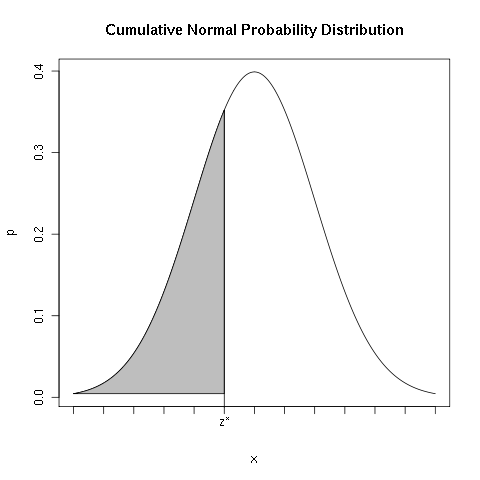
\includegraphics[height=3.25cm]{img/cummulativeDist}

\begin{tabular}{l|llllllllll}
     & 0.00   & 0.01   & 0.02   & 0.03   & 0.04   & 0.05   & 0.06   & 0.07   & 0.08  & 0.09 \\ \hline
-3.4 & 0.0003 & 0.0003 & 0.0003 & 0.0003 & 0.0003 & 0.0003 & 0.0003 & 0.0003 & 0.0003 & 0.0002 \\\arrayrulecolor{light-gray}\hline\arrayrulecolor{black} 
-3.3 & 0.0005 & 0.0005 & 0.0005 & 0.0004 & 0.0004 & 0.0004 & 0.0004 & 0.0004 & 0.0004 & 0.0003 \\\arrayrulecolor{light-gray}\hline\arrayrulecolor{black} 
-3.2 & 0.0007 & 0.0007 & 0.0006 & 0.0006 & 0.0006 & 0.0006 & 0.0006 & 0.0005 & 0.0005 & 0.0005 \\\arrayrulecolor{light-gray}\hline\arrayrulecolor{black} 
-3.1 & 0.0010 & 0.0009 & 0.0009 & 0.0009 & 0.0008 & 0.0008 & 0.0008 & 0.0008 & 0.0007 & 0.0007 \\\arrayrulecolor{light-gray}\hline\arrayrulecolor{black} 
-3.0 & 0.0013 & 0.0013 & 0.0013 & 0.0012 & 0.0012 & 0.0011 & 0.0011 & 0.0011 & 0.0010 & 0.0010 \\\arrayrulecolor{light-gray}\hline\arrayrulecolor{black} 
-2.9 & 0.0019 & 0.0018 & 0.0018 & 0.0017 & 0.0016 & 0.0016 & 0.0015 & 0.0015 & 0.0014 & 0.0014 \\\arrayrulecolor{light-gray}\hline\arrayrulecolor{black} 
-2.8 & 0.0026 & 0.0025 & 0.0024 & 0.0023 & 0.0023 & 0.0022 & 0.0021 & 0.0021 & 0.0020 & 0.0019 \\\arrayrulecolor{light-gray}\hline\arrayrulecolor{black} 
-2.7 & 0.0035 & 0.0034 & 0.0033 & 0.0032 & 0.0031 & 0.0030 & 0.0029 & 0.0028 & 0.0027 & 0.0026 \\\arrayrulecolor{light-gray}\hline\arrayrulecolor{black} 
-2.6 & 0.0047 & 0.0045 & 0.0044 & 0.0043 & 0.0041 & 0.0040 & 0.0039 & 0.0038 & 0.0037 & 0.0036 \\\arrayrulecolor{light-gray}\hline\arrayrulecolor{black} 
-2.5 & 0.0062 & 0.0060 & 0.0059 & 0.0057 & 0.0055 & 0.0054 & 0.0052 & 0.0051 & 0.0049 & 0.0048 \\\arrayrulecolor{light-gray}\hline\arrayrulecolor{black} 
-2.4 & 0.0082 & 0.0080 & 0.0078 & 0.0075 & 0.0073 & 0.0071 & 0.0069 & 0.0068 & 0.0066 & 0.0064 \\\arrayrulecolor{light-gray}\hline\arrayrulecolor{black} 
-2.3 & 0.0107 & 0.0104 & 0.0102 & 0.0099 & 0.0096 & 0.0094 & 0.0091 & 0.0089 & 0.0087 & 0.0084 \\\arrayrulecolor{light-gray}\hline\arrayrulecolor{black} 
-2.2 & 0.0139 & 0.0136 & 0.0132 & 0.0129 & 0.0125 & 0.0122 & 0.0119 & 0.0116 & 0.0113 & 0.0110 \\\arrayrulecolor{light-gray}\hline\arrayrulecolor{black} 
-2.1 & 0.0179 & 0.0174 & 0.0170 & 0.0166 & 0.0162 & 0.0158 & 0.0154 & 0.0150 & 0.0146 & 0.0143 \\\arrayrulecolor{light-gray}\hline\arrayrulecolor{black} 
-2.0 & 0.0228 & 0.0222 & 0.0217 & 0.0212 & 0.0207 & 0.0202 & 0.0197 & 0.0192 & 0.0188 & 0.0183 \\\arrayrulecolor{light-gray}\hline\arrayrulecolor{black} 
-1.9 & 0.0287 & 0.0281 & 0.0274 & 0.0268 & 0.0262 & 0.0256 & 0.0250 & 0.0244 & 0.0239 & 0.0233 \\\arrayrulecolor{light-gray}\hline\arrayrulecolor{black} 
-1.8 & 0.0359 & 0.0351 & 0.0344 & 0.0336 & 0.0329 & 0.0322 & 0.0314 & 0.0307 & 0.0301 & 0.0294 \\\arrayrulecolor{light-gray}\hline\arrayrulecolor{black} 
-1.7 & 0.0446 & 0.0436 & 0.0427 & 0.0418 & 0.0409 & 0.0401 & 0.0392 & 0.0384 & 0.0375 & 0.0367 \\\arrayrulecolor{light-gray}\hline\arrayrulecolor{black} 
-1.6 & 0.0548 & 0.0537 & 0.0526 & 0.0516 & 0.0505 & 0.0495 & 0.0485 & 0.0475 & 0.0465 & 0.0455 \\\arrayrulecolor{light-gray}\hline\arrayrulecolor{black} 
-1.5 & 0.0668 & 0.0655 & 0.0643 & 0.0630 & 0.0618 & 0.0606 & 0.0594 & 0.0582 & 0.0571 & 0.0559 \\\arrayrulecolor{light-gray}\hline\arrayrulecolor{black} 
-1.4 & 0.0808 & 0.0793 & 0.0778 & 0.0764 & 0.0749 & 0.0735 & 0.0721 & 0.0708 & 0.0694 & 0.0681 \\\arrayrulecolor{light-gray}\hline\arrayrulecolor{black} 
-1.3 & 0.0968 & 0.0951 & 0.0934 & 0.0918 & 0.0901 & 0.0885 & 0.0869 & 0.0853 & 0.0838 & 0.0823 \\\arrayrulecolor{light-gray}\hline\arrayrulecolor{black} 
-1.2 & 0.1151 & 0.1131 & 0.1112 & 0.1093 & 0.1075 & 0.1056 & 0.1038 & 0.1020 & 0.1003 & 0.0985 \\\arrayrulecolor{light-gray}\hline\arrayrulecolor{black} 
-1.1 & 0.1357 & 0.1335 & 0.1314 & 0.1292 & 0.1271 & 0.1251 & 0.1230 & 0.1210 & 0.1190 & 0.1170 \\\arrayrulecolor{light-gray}\hline\arrayrulecolor{black} 
-1.0 & 0.1587 & 0.1562 & 0.1539 & 0.1515 & 0.1492 & 0.1469 & 0.1446 & 0.1423 & 0.1401 & 0.1379 \\\arrayrulecolor{light-gray}\hline\arrayrulecolor{black} 
-0.9 & 0.1841 & 0.1814 & 0.1788 & 0.1762 & 0.1736 & 0.1711 & 0.1685 & 0.1660 & 0.1635 & 0.1611 \\\arrayrulecolor{light-gray}\hline\arrayrulecolor{black} 
-0.8 & 0.2119 & 0.2090 & 0.2061 & 0.2033 & 0.2005 & 0.1977 & 0.1949 & 0.1922 & 0.1894 & 0.1867 \\\arrayrulecolor{light-gray}\hline\arrayrulecolor{black} 
-0.7 & 0.2420 & 0.2389 & 0.2358 & 0.2327 & 0.2296 & 0.2266 & 0.2236 & 0.2206 & 0.2177 & 0.2148 \\\arrayrulecolor{light-gray}\hline\arrayrulecolor{black} 
-0.6 & 0.2743 & 0.2709 & 0.2676 & 0.2643 & 0.2611 & 0.2578 & 0.2546 & 0.2514 & 0.2483 & 0.2451 \\\arrayrulecolor{light-gray}\hline\arrayrulecolor{black} 
-0.5 & 0.3085 & 0.3050 & 0.3015 & 0.2981 & 0.2946 & 0.2912 & 0.2877 & 0.2843 & 0.2810 & 0.2776 \\\arrayrulecolor{light-gray}\hline\arrayrulecolor{black} 
-0.4 & 0.3446 & 0.3409 & 0.3372 & 0.3336 & 0.3300 & 0.3264 & 0.3228 & 0.3192 & 0.3156 & 0.3121 \\\arrayrulecolor{light-gray}\hline\arrayrulecolor{black} 
-0.3 & 0.3821 & 0.3783 & 0.3745 & 0.3707 & 0.3669 & 0.3632 & 0.3594 & 0.3557 & 0.3520 & 0.3483 \\\arrayrulecolor{light-gray}\hline\arrayrulecolor{black} 
-0.2 & 0.4207 & 0.4168 & 0.4129 & 0.4090 & 0.4052 & 0.4013 & 0.3974 & 0.3936 & 0.3897 & 0.3859 \\\arrayrulecolor{light-gray}\hline\arrayrulecolor{black} 
-0.1 & 0.4602 & 0.4562 & 0.4522 & 0.4483 & 0.4443 & 0.4404 & 0.4364 & 0.4325 & 0.4286 & 0.4247 \\\arrayrulecolor{light-gray}\hline\arrayrulecolor{black} 
-0.0 & 0.5000 & 0.4960 & 0.4920 & 0.4880 & 0.4840 & 0.4801 & 0.4761 & 0.4721 & 0.4681 & 0.4641 \\\arrayrulecolor{light-gray}\hline\arrayrulecolor{black} 
\end{tabular}


\clearpage
 Approximation of the cumulative distribution for the standard normal distribution. 
 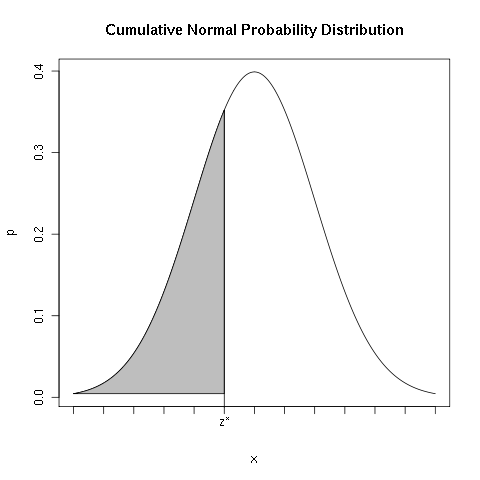
\includegraphics[height=3.25cm]{img/cummulativeDist}

 \begin{tabular}{l|llllllllll}
     & 0.00   & 0.01   & 0.02   & 0.03   & 0.04   & 0.05   & 0.06   & 0.07   & 0.08  & 0.09 \\ \hline
0.0 & 0.5000 & 0.5040 & 0.5080 & 0.5120 & 0.5160 & 0.5199 & 0.5239 & 0.5279 & 0.5319 & 0.5359 \\\arrayrulecolor{light-gray}\hline\arrayrulecolor{black} 
0.1 & 0.5398 & 0.5438 & 0.5478 & 0.5517 & 0.5557 & 0.5596 & 0.5636 & 0.5675 & 0.5714 & 0.5753 \\\arrayrulecolor{light-gray}\hline\arrayrulecolor{black} 
0.2 & 0.5793 & 0.5832 & 0.5871 & 0.5910 & 0.5948 & 0.5987 & 0.6026 & 0.6064 & 0.6103 & 0.6141 \\\arrayrulecolor{light-gray}\hline\arrayrulecolor{black} 
0.3 & 0.6179 & 0.6217 & 0.6255 & 0.6293 & 0.6331 & 0.6368 & 0.6406 & 0.6443 & 0.6480 & 0.6517 \\\arrayrulecolor{light-gray}\hline\arrayrulecolor{black} 
0.4 & 0.6554 & 0.6591 & 0.6628 & 0.6664 & 0.6700 & 0.6736 & 0.6772 & 0.6808 & 0.6844 & 0.6879 \\\arrayrulecolor{light-gray}\hline\arrayrulecolor{black} 
0.5 & 0.6915 & 0.6950 & 0.6985 & 0.7019 & 0.7054 & 0.7088 & 0.7123 & 0.7157 & 0.7190 & 0.7224 \\\arrayrulecolor{light-gray}\hline\arrayrulecolor{black} 
0.6 & 0.7257 & 0.7291 & 0.7324 & 0.7357 & 0.7389 & 0.7422 & 0.7454 & 0.7486 & 0.7517 & 0.7549 \\\arrayrulecolor{light-gray}\hline\arrayrulecolor{black} 
0.7 & 0.7580 & 0.7611 & 0.7642 & 0.7673 & 0.7704 & 0.7734 & 0.7764 & 0.7794 & 0.7823 & 0.7852 \\\arrayrulecolor{light-gray}\hline\arrayrulecolor{black} 
0.8 & 0.7881 & 0.7910 & 0.7939 & 0.7967 & 0.7995 & 0.8023 & 0.8051 & 0.8078 & 0.8106 & 0.8133 \\\arrayrulecolor{light-gray}\hline\arrayrulecolor{black} 
0.9 & 0.8159 & 0.8186 & 0.8212 & 0.8238 & 0.8264 & 0.8289 & 0.8315 & 0.8340 & 0.8365 & 0.8389 \\\arrayrulecolor{light-gray}\hline\arrayrulecolor{black} 
1.0 & 0.8413 & 0.8438 & 0.8461 & 0.8485 & 0.8508 & 0.8531 & 0.8554 & 0.8577 & 0.8599 & 0.8621 \\\arrayrulecolor{light-gray}\hline\arrayrulecolor{black} 
1.1 & 0.8643 & 0.8665 & 0.8686 & 0.8708 & 0.8729 & 0.8749 & 0.8770 & 0.8790 & 0.8810 & 0.8830 \\\arrayrulecolor{light-gray}\hline\arrayrulecolor{black} 
1.2 & 0.8849 & 0.8869 & 0.8888 & 0.8907 & 0.8925 & 0.8944 & 0.8962 & 0.8980 & 0.8997 & 0.9015 \\\arrayrulecolor{light-gray}\hline\arrayrulecolor{black} 
1.3 & 0.9032 & 0.9049 & 0.9066 & 0.9082 & 0.9099 & 0.9115 & 0.9131 & 0.9147 & 0.9162 & 0.9177 \\\arrayrulecolor{light-gray}\hline\arrayrulecolor{black} 
1.4 & 0.9192 & 0.9207 & 0.9222 & 0.9236 & 0.9251 & 0.9265 & 0.9279 & 0.9292 & 0.9306 & 0.9319 \\\arrayrulecolor{light-gray}\hline\arrayrulecolor{black} 
1.5 & 0.9332 & 0.9345 & 0.9357 & 0.9370 & 0.9382 & 0.9394 & 0.9406 & 0.9418 & 0.9429 & 0.9441 \\\arrayrulecolor{light-gray}\hline\arrayrulecolor{black} 
1.6 & 0.9452 & 0.9463 & 0.9474 & 0.9484 & 0.9495 & 0.9505 & 0.9515 & 0.9525 & 0.9535 & 0.9545 \\\arrayrulecolor{light-gray}\hline\arrayrulecolor{black} 
1.7 & 0.9554 & 0.9564 & 0.9573 & 0.9582 & 0.9591 & 0.9599 & 0.9608 & 0.9616 & 0.9625 & 0.9633 \\\arrayrulecolor{light-gray}\hline\arrayrulecolor{black} 
1.8 & 0.9641 & 0.9649 & 0.9656 & 0.9664 & 0.9671 & 0.9678 & 0.9686 & 0.9693 & 0.9699 & 0.9706 \\\arrayrulecolor{light-gray}\hline\arrayrulecolor{black} 
1.9 & 0.9713 & 0.9719 & 0.9726 & 0.9732 & 0.9738 & 0.9744 & 0.9750 & 0.9756 & 0.9761 & 0.9767 \\\arrayrulecolor{light-gray}\hline\arrayrulecolor{black} 
2.0 & 0.9772 & 0.9778 & 0.9783 & 0.9788 & 0.9793 & 0.9798 & 0.9803 & 0.9808 & 0.9812 & 0.9817 \\\arrayrulecolor{light-gray}\hline\arrayrulecolor{black} 
2.1 & 0.9821 & 0.9826 & 0.9830 & 0.9834 & 0.9838 & 0.9842 & 0.9846 & 0.9850 & 0.9854 & 0.9857 \\\arrayrulecolor{light-gray}\hline\arrayrulecolor{black} 
2.2 & 0.9861 & 0.9864 & 0.9868 & 0.9871 & 0.9875 & 0.9878 & 0.9881 & 0.9884 & 0.9887 & 0.9890 \\\arrayrulecolor{light-gray}\hline\arrayrulecolor{black} 
2.3 & 0.9893 & 0.9896 & 0.9898 & 0.9901 & 0.9904 & 0.9906 & 0.9909 & 0.9911 & 0.9913 & 0.9916 \\\arrayrulecolor{light-gray}\hline\arrayrulecolor{black} 
2.4 & 0.9918 & 0.9920 & 0.9922 & 0.9925 & 0.9927 & 0.9929 & 0.9931 & 0.9932 & 0.9934 & 0.9936 \\\arrayrulecolor{light-gray}\hline\arrayrulecolor{black} 
2.5 & 0.9938 & 0.9940 & 0.9941 & 0.9943 & 0.9945 & 0.9946 & 0.9948 & 0.9949 & 0.9951 & 0.9952 \\\arrayrulecolor{light-gray}\hline\arrayrulecolor{black} 
2.6 & 0.9953 & 0.9955 & 0.9956 & 0.9957 & 0.9959 & 0.9960 & 0.9961 & 0.9962 & 0.9963 & 0.9964 \\\arrayrulecolor{light-gray}\hline\arrayrulecolor{black} 
2.7 & 0.9965 & 0.9966 & 0.9967 & 0.9968 & 0.9969 & 0.9970 & 0.9971 & 0.9972 & 0.9973 & 0.9974 \\\arrayrulecolor{light-gray}\hline\arrayrulecolor{black} 
2.8 & 0.9974 & 0.9975 & 0.9976 & 0.9977 & 0.9977 & 0.9978 & 0.9979 & 0.9979 & 0.9980 & 0.9981 \\\arrayrulecolor{light-gray}\hline\arrayrulecolor{black} 
2.9 & 0.9981 & 0.9982 & 0.9982 & 0.9983 & 0.9984 & 0.9984 & 0.9985 & 0.9985 & 0.9986 & 0.9986 \\\arrayrulecolor{light-gray}\hline\arrayrulecolor{black} 
3.0 & 0.9987 & 0.9987 & 0.9987 & 0.9988 & 0.9988 & 0.9989 & 0.9989 & 0.9989 & 0.9990 & 0.9990 \\\arrayrulecolor{light-gray}\hline\arrayrulecolor{black} 
3.1 & 0.9990 & 0.9991 & 0.9991 & 0.9991 & 0.9992 & 0.9992 & 0.9992 & 0.9992 & 0.9993 & 0.9993 \\\arrayrulecolor{light-gray}\hline\arrayrulecolor{black} 
3.2 & 0.9993 & 0.9993 & 0.9994 & 0.9994 & 0.9994 & 0.9994 & 0.9994 & 0.9995 & 0.9995 & 0.9995 \\\arrayrulecolor{light-gray}\hline\arrayrulecolor{black} 
3.3 & 0.9995 & 0.9995 & 0.9995 & 0.9996 & 0.9996 & 0.9996 & 0.9996 & 0.9996 & 0.9996 & 0.9997 \\\arrayrulecolor{light-gray}\hline\arrayrulecolor{black} 
3.4 & 0.9997 & 0.9997 & 0.9997 & 0.9997 & 0.9997 & 0.9997 & 0.9997 & 0.9997 & 0.9997 & 0.9998 \\\arrayrulecolor{light-gray}\hline\arrayrulecolor{black} 
\end{tabular}

\clearpage

\begin{problem}

  \item Find each of the following probabilities for the standard
    normal.
    \begin{subproblem}
      \item $p(Z \leq 0.37)$
        \vfill
      \item $p(Z \leq -0.72)$
        \vfill
      \item $p(Z \leq -2.6)$
        \vfill
      \item $p(Z \leq 0.5)$
        \vfill
      \item $p(Z \geq 0.5)$
        \vfill
      \item $p(Z \leq -0.5)$
        \vfill
      \item $p(Z \geq -0.5)$
        \vfill
      \item $p(Z < 0.5)$
        \vfill
    \end{subproblem}

    \clearpage

  \item Find each of the following probabilities for the standard
    normal.
    \begin{subproblem}
      \item $p((Z \leq 0.37) \mathrm{~and~} (Z \geq -0.37) )$
        \vfill
      \item $p((Z \leq 1.91) \mathrm{~and~} (Z \geq -2.11) )$
        \vfill
      \item $p((Z \leq -2.67) \mathrm{~or~} (Z \geq 2.67) )$
        \vfill
      \item $p((Z \leq -1.17) \mathrm{~or~} (Z \geq 0.71) )$
        \vfill
    \end{subproblem}

  \item For each problem below determine an approximation for $Z_0$
    \begin{subproblem}
      \item $p(Z < Z_0) = 0.05 $
        \vfill
      \item $p(Z < Z_0) = 0.75 $
        \vfill
      \item $p(Z < Z_0) = 0.95 $
        \vfill
      \item $p(Z > Z_0) = 0.25 $
        \vfill
      \item $p(Z > Z_0) = 0.95 $
        \vfill
      \item $p((Z \leq -Z_0) \mathrm{~or~} (Z \geq Z_0) ) = 0.05$
        (Assume that $Z_0>0$.)
        \vfill
      \item $p((Z \geq -Z_0) \mathrm{~and~} (Z \leq Z_0) ) = 0.95$
        (Assume that $Z_0>0$.)
        \vfill
    \end{subproblem}

    \clearpage

\item Financial analysts who make forecasts are categorized as either
  being ``buy-side'' or ``sell-side'' analysts. It is estimated that
  the forecast error for buy-side analysts is 0.85 with a standard
  deviation of 1.93. It is estimated that the forecast error for
  sell-side analysts is -0.05 with a standard deviation of
  0.85. Sketch plots for the distributions for the two types of
  analysts assuming the errors are normally distributed.  Determine
  the following probabilities

  \begin{subproblem}
    \item The probability that a buy-side analyst's error is more than
      1.1.
      \vfill
    \item The probability that a sell-side analyst's error is more than
      1.1.
      \vfill
    \item The probability that a buy-side analyst's error is less than
      -1.1.
      \vfill
    \item The probability that a sell-side analyst's error is less than
      -1.1.
      \vfill
  \end{subproblem}



  
\end{problem}

           % 9 and 10


\chapter{Descriptive Statistics}
\preClass{Counting Number of Approaches}


\begin{problem}
\item Examples of uniform probability distributions.

  \begin{subproblem}
  \item 
    \begin{eqnarray}
      y & = 3x + 4.
    \end{eqnarray}
    \vfill
  \end{subproblem}


\end{problem}


\actTitle{Data Collection} 


\begin{problem}

\item An investment bank will conduct a stress test to determine how
  it can react to swings in the markets. As part of the test the
  managers within different offices are asked the following questions:
  \begin{itemize}
  \item What is the total balance in your reserve accounts?
  \item What is the mean error in your return projections over the
    past year?
  \item On a scale from one to five how would you rate your current
    risk? (One means low risk and five is high risk.)
  \item On a scale from one to five how would you rate your current
    operating process? (One means inefficient and five is highly
    efficient.)
  \item When evaluating a fund which aspects of the fund are most
    important in terms of deciding your investment levels? (Circle all
    that apply: \\
    Price; Derivatives; Credit Scoring; Financial Activity; Open
    Options; Dynamic Financial Analysis Projections.
  \end{itemize}

  For each question above determine the nature of the data that will
  result from the survey. Determine if it qualitative, quantitative,
  and if it is quantitative determine if it is ordinal or continuous
  data.

  \vfill

  \clearpage

\item The human resources department examines applications for
  employment. Each applicant answers a number of questions:

  \begin{itemize}
  \item What is your gender? 
  \item What is your age?
  \item What is your racial background?
  \item What is your GPA?
  \item What is your total number of credit hours completed?
  \item What is your expected salary?
  \end{itemize}

  For each question above determine the nature of the data that will
  result from the survey. Determine if it qualitative, quantitative,
  and if it is quantitative determine if it is ordinal or continuous
  data.

  \vfill

  \clearpage

\item Firms that are in bankruptcy are randomly sampled. For each firm
  the reorganization plan in place and the time they have been in
  bankruptcy (in months) is recorded. The data is given below:

  \begin{tabular}{ll|ll|ll} % @{\hspace{3em}
    Plan & Time  (months) & 
    Plan & Time  (months) & 
    Plan & Time  (months)\\ \hline
    None    & 10.1 & Prepack & 4.7  & Prepack & 7.3 \\
    Prepack & 6.7  & Prepack & 7    & Joint   & 7.4 \\
    None    & 10.5 & Joint   & 3.3  & Prepack & 5.5 \\
    Joint   & 5.8  & None    & 11.2 & Joint   & 7.4 \\
    Joint   & 7.5  & Prepack & 8.6  & Joint   & 7.2 
  \end{tabular}

  \begin{subproblem}
  \item Determine the frequency of firms using each type of bankruptcy
    plan.
    \vfill
  \item Determine the frequency of firms whose time in bankruptcy is less
    than 6 months. 
    \vfill
  \item For each type of plan determine the frequency of firms whose
    time in bankruptcy is less than 6 months, between 6 and 8 months,
    between 8 and 10 months, and between 10 and 12 months. Express the
    results as a table with each row being one of the plan types, and
    the columns are the time in bankruptcy.
    \vfill
  \end{subproblem}


\clearpage

\item The human resources division conducts a  survey for people who
  have applied for a position in the past year. Each person is asked a
  number of questions. Two questions in particular are examined:
  \begin{enumerate}
  \item On a scale from one to four how would you rate the feedback
    you received from our corporation? (One is poor and four is
    excellent.)
  \item On a scale from one to four how would rate your overall
    experience?  (One is poor and four is excellent.)
  \end{enumerate}

  \begin{tabular}{ll|ll|ll|ll|ll} % @{\hspace{3em}
    Q1 & Q2 & Q1 & Q2 & Q1 & Q2 & Q1 & Q2 & Q1 & Q2 \\ \hline
    2 & 3 & 4 & 4 & 4 & 2 & 3 & 4 & 2 & 3 \\
    3 & 3 & 1 & 3 & 4 & 4 & 2 & 4 & 4 & 3 \\
    4 & 1 & 1 & 1 & 4 & 3 & 2 & 2 & 3 & 3 \\
    4 & 1 & 3 & 2 & 4 & 4 & 3 & 3 & 4 & 2 \\
    4 & 3 & 3 & 3 & 4 & 3 & 3 & 1 & 1 & 2
  \end{tabular}

  \begin{subproblem}
  \item Determine the frequency of people answering 4 on question one
    and 4 on question two.
    \vspace{2em}
  \item Make a table in which each row corresponds to the possible
    answers on question one, and each column corresponds to the possible
    answers on question two. For each entry in the table determine the
    frequency of occurrences for the number of people with the given
    pair of responses.

    \vfill

  \end{subproblem}

  
\end{problem}


\actTitle{Experimental Design} 

\begin{problem}
\item The mean sales for facilities will be examined. Your firm's
  facilities can be categorized as being stand alone, in a strip mall,
  or in an enclosed mall. The stores can also be categorized as being
  boutique, small, or large. Finally the stores can be categorizes as
  being for appointment, open, office, or call center.
    \begin{subproblem}
      \item How many different overall categories are there?
        \vfill
      \item If the study requires that there will be 20 stores for
        each category how many stores must be chosen?
        \vfill
      \item Describe the type of data that will be calculated for each
        category of store.
        \vspace{2em}
    \end{subproblem}

\clearpage

\item The effectiveness of a rehabilitation treatment after surgery
  will be tested. The team wishes to test the effectiveness for one,
  two, and three sessions per day. They also wish to test the
  effectiveness for sessions lasting 30 minutes, 60 minutes, 75
  minutes, and 90 minutes. Finally, the treatment can be given over a
  one week period or a two week period. At the end of the treatment
  each patient's improvement is rated as being poor, adequate, or excellent.
    \begin{subproblem}
      \item How many different overall categories are there?
        \vfill
      \item If the study requires that there will be 15 patients for
        each category how many patients must be chosen?
        \vfill
      \item Describe the type of data that will be calculated for each
        category.
        \vspace{2em}
    \end{subproblem}

\clearpage

\item A study will be conducted to determine the cost of vandalism
  over a year. Your firm will randomly select stores and ask how much
  money was spent in repairs due to vandalism. It is estimated that
  the standard deviation of the sample mean for the costs is
  \begin{eqnarray*}
    \hat{\sigma} & = & \frac{120.5}{\sqrt{n}},
  \end{eqnarray*}
  where $n$ is the number of stores to sample.

  \begin{subproblem}
    \item Determine how many samples are required if the standard
      deviation of the sample mean should be 10.0.

      \vfill

    \item Determine how many samples are required if the standard
      deviation of the sample mean should be 5.0.

      \vfill

    \item Repeat the previous calculations if the standard deviation
      for the sample mean is
      \begin{eqnarray*}
        \hat{\sigma} & = & \frac{130.5}{\sqrt{n}}.
      \end{eqnarray*}

      \vfill


  \end{subproblem}

\end{problem}


%  LocalWords:  Prepack
           % 11 and 12
\preClass{Counting Number of Approaches}


\begin{problem}
\item Examples of uniform probability distributions.

  \begin{subproblem}
  \item 
    \begin{eqnarray}
      y & = 3x + 4.
    \end{eqnarray}
    \vfill
  \end{subproblem}


\end{problem}


\actTitle{Plotting Discrete Data} 


\begin{problem}

\item A new product is tested in the Midwest. People are chosen at
  random and asked to try the product. They are asked to provide their
  initial reaction on a scale from 1 to 5, where 1 means they would
  not purchase it and 5 means they are strongly wish to purchase the
  product.

  Their results are given below:\\
  \begin{tabular}{rrrrrrrrrrrrrrrr}
    3 & 3 & 4 & 3 & 2 & 2 & 4 & 3 &
    1 & 4 & 3 & 3 & 3 & 3 & 4 & 4 \\
    4 & 3 & 3 & 3 & 3 & 3 & 4 & 3 &
    4 & 3 & 3 & 4 & 3 & 3 & 4 & 2 \\
  \end{tabular}

  \begin{subproblem}
  \item Determine the frequency of the occurences for each possible
    response.
    \vfill
  \item Make a rough sketch of a bar plot with the responses given in
    order (1, 2, 3, 4, and 5).
    \vfill
    \clearpage
  \item Make a rough sketch of the Pareto plot for the responses.
    \vfill
  \item Provide a description of the data. What are the important features?
    \vspace{10em}
  \end{subproblem}

\clearpage

\item A clinic wishes to test a therapy for children that they have
  not used in the past. They choose a number of patients at random and
  use the Face, Legs, Activity, Cry, Consolability scale (FLACC) to
  assess the patients' pain levels. (The FLACC scale provides a number
  between 0 and 10.) After the study they have the following
  observations.

  Their results are given below:\\
  \begin{tabular}{rrrrrrrrrrrrrrrr}
    5 & 7 & 6 & 6 & 8 & 5 & 6 & 5 &
    4 & 7 & 8 & 5 & 6 & 5 & 8 & 3 \\
    6 & 6 & 5 & 6 & 4 & 6 & 5 & 4 &
    5 & 5 & 3 & 6 & 8 & 5 & 6 & 4 \\
    8 & 6 & 8 & 5 & 6 & 8 & 3 & 6 
  \end{tabular}

  \begin{subproblem}
  \item Determine the frequency of the occurences for each possible
    response.
    \vfill
  \item Make a rough sketch of a bar plot with the responses given in
    order (0, 1, 2, 3, through 10).
    \vfill
    \clearpage
  \item Make a rough sketch of the Pareto plot for the responses.
    \vfill
  \item Provide a description of the data. What are the important features?
    \vspace{5em}
  \end{subproblem}

\clearpage

\item Concerns about costs associated with insurance processing fees
  has been raised by the Human Resources Department. They chose a
  random group of people and rated the associated costs as being L
  (low), M (medium), or H (high). Each person was then determined to
  be either a S (smoker) or NS (non-smoker).

  Their results are given below:\\
  \begin{tabular}{rr|rr|rr|rr|rr|rr|rr|rr}
    H & S  & M & S  & M & NS & L & NS & L & S  & M & NS & M & S  & M & NS  \\
    M & S  & M & NS & M & NS & H & S  & L & NS & L & S  & M & NS & L & S  \\
    L & NS & M & S  & H & S  & L & NS & M & S  & M & NS & L & NS & H & NS \\
    M & NS & M & NS & M & S  & M & S  & M & NS & M & NS & M & NS & L & NS \\
    M & S  & L & NS & L & NS & L & S  & M & NS & M & S  & H & S  & L & S 
  \end{tabular}

  \begin{subproblem}
    \item Determine the frequency of occurrences for  each possible
      combination.
      \vfill
    \item Arrange the frequencies into a table with the costs arranged
      in rows and the smoking status in the columns.
      \vfill
  \end{subproblem}
  
\end{problem}

\actTitle{Plotting Continuous Data} 

\begin{problem}
\item The calls made by people in a call center are monitored. The
  total amount of time for each call is observed, and a number of
  calls are chosen at random.

    The call times are given in the table below:\\
    \begin{tabular}{rrrrrrrrrrrr}
      37.9 & 31.9 & 21.4 & 24.7 & 34.3 & 47.5 & 27.6 & 16.4 &
      28.7 & 31.0 & 32.6 & 37.4 \\
      31.0 & 25.5 & 35.9 & 35.1 & 27.3 & 37.9 & 31.6 & 29.0 &
      18.2 & 15.0 & 33.4 & 42.8  \\
      36.1 & 28.2 & 19.6 & 35.2 & 31.1 & 30.5 & 34.9 & 22.8 &
      29.2 & 32.0 & 28.5 & 32.9 \\
      33.9 & 25.6 & 28.6 & 26.3
    \end{tabular}
    
    \begin{subproblem}
      \item Make a stem-leaf plot of the data by rounding the numbers.
        \vfill
      \item Make a stem-leaf plot of the data by truncating the
        numbers.
        \vfill
        \clearpage
      \item Sketch a histogram using an interval width of 5.
        \vfill
      \item Sketch a histogram using an interval width of 10.
        \vfill
      \item Provide a description of the data. What are the important features?
        \vspace{5em}
    \end{subproblem}

\clearpage

  \item The heart rates in beats per minute are measured for a group
    of adults. 

    The results are given below:\\
    \begin{tabular}{rrrrrrrrrrrrr}
      73.3 & 70.8 & 75.8 & 67.5 & 67.6 & 69.0 & 73.0 & 69.8 & 70.8 & 70.5 & 69.2 & 70.1 & 69.7 \\
      69.7 & 73.8 & 73.7 & 68.9 & 69.7 & 67.9 & 66.5 & 68.7 & 72.1 & 70.1 & 67.9 & 72.1 & 66.9 \\
      66.9 & 70.2 & 73.0 & 73.0 & 71.6 & 65.7 & 72.0 & 70.9 & 73.0 & 69.8 & 66.0 & 65.9 & 71.3 \\
      71.3 & 70.2 & 68.0 & 72.3 
    \end{tabular}
    
    \begin{subproblem}
      \item Make a stem-leaf plot of the data by rounding the numbers.
        \vfill
      \item Make a stem-leaf plot of the data by truncating the
        numbers.
        \vfill
        \clearpage
      \item Sketch a histogram using an interval width of 5.
        \vfill
      \item Sketch a histogram using an interval width of 10.
        \vfill
      \item Provide a description of the data. What are the important features?
        \vspace{5em}
    \end{subproblem}

\clearpage

\item The heart rates in beats per minute are measured for a different
  group of adults.

    The results are given below:\\
    \begin{tabular}{rrrrrrrrrrrrr}
      75.4 & 76.8 & 73.9 & 72.4 & 70.9 & 70.4 & 75.4 & 79.3 & 77.0 & 77.6 & 75.1 & 74.4 & 75.1 \\
      75.1 & 73.7 & 78.9 & 73.8 & 74.7 & 82.3 & 68.8 & 76.4 & 75.7 & 70.5 & 78.0 & 75.4 & 81.1 \\
      81.1 & 71.0 & 71.1 & 76.0 & 76.1 & 78.1 & 81.3 & 67.2 & 74.6 & 74.2 & 76.2 & 72.4 & 72.4 \\
      72.4 & 71.4 & 71.7 & 69.4
    \end{tabular}
    
    \begin{subproblem}
      \item Make a stem-leaf plot of the data by rounding the numbers.
        \vfill
      \item Sketch a histogram using an interval width of 5.
        \vfill
        \clearpage
      \item Sketch a histogram using an interval width of 10.
        \vfill
      \item Is this group of people's heart rate different from the
        previous group? Justify your conclusions.

        \vspace{4em}
    \end{subproblem}


\end{problem}

                     % 13 and 14
\preClass{Calculating Sample Means}


\begin{problem}
\item Examples of calculating sample means.

  \begin{subproblem}
  \item 
    \begin{eqnarray}
      y & = 3x + 4.
    \end{eqnarray}
    \vfill
  \end{subproblem}


\end{problem}


\actTitle{Calculating Sample Means and Sample Standard Deviations} 


\begin{problem}

\item The  questions below refer to the following set of data: \\
  \begin{tabular}{rrrrrrrr}
    9 & 14.3 & 11.2 & 12.7 & 16.8 & 12.8 & 9.7 & 23.2
  \end{tabular}

  \begin{subproblem}
  \item Make a sketch of a strip chart for the data. Provide a brief
    description about the data and note any patterns.

    \vspace{8em}


  \item Calculate the sample mean, sample standard deviation, and the
    coefficient of variation for the data.

    \vfill

  \item Remove the largest number and then calculate the sample mean,
    the sample standard deviation, and the coefficient of variation
    for the data.

    \vfill

  \item Calculate the percent difference in the values of the sample
    mean and sample standard deviations.

    \vspace{4em}

  \end{subproblem}

  \clearpage

\item A random collection of firms that have filed for chapter 7 bankruptcy will
  be polled and asked how long they have been in bankruptcy. Your
  group believes that the mean length of time in months is 2.3 months
  with a standard deviation of 0.6 months.

  \begin{subproblem}
  \item If $X$ is a random variable with mean $\mu$ and standard
    devitation $\sigma$ then Chebychev's inequality is
    \begin{eqnarray*}
      p\left( -k \sigma \leq X - \mu \leq k \sigma \right) \leq \frac{1}{k^2}.
    \end{eqnarray*}
    Your group plans on polling one-hundred firms. How many of the
    times do you expect to be between 2.0 months and 2.6 months.
    \marginnote{Hint: make a sketch of the real line marking the mean
      and the left and right bounds.}[0cm]

    \vfill

  \item Your group plans on polling one-hundred firms. How many of the
    times do you expect to be between 1.1 months and 3.5 months.

    \vfill

  \item Your group plans on polling one-hundred firms. How many of the
    times do you expect to be between 0.8 months and 3.8 months.

    \vfill

    \clearpage

  \item Your group takes an initial poll, and the results are given
    below. Determine the sample mean and sample standard deviation of
    the sample. \\
    \begin{tabular}{rrrrrrrr}
      3.1 & 1.8 & 1.6 & 3.0 & 3.0 & 2.7 & 3.2 & 2.7
    \end{tabular}

    \vfill

  \item Your group takes a second poll, and the results are given
    below. Determine the sample mean and sample standard deviation of
    the sample. \\
    \begin{tabular}{rrrrrrrr}
      2.6 & 2.4 & 3.0 & 2.7 & 1.9 & 2.3 & 2.8 & 2.7
    \end{tabular}

    \vfill

  \item Why are the results different?

    \vspace{4em}

  \end{subproblem}

\end{problem}

\actTitle{Calculating The Five Point Summary and Box Plots} 

\begin{problem}

\item We will re-examine the data used in the first problem of the
  previous activity. The  questions below refer to the following set of data: \\
  \begin{tabular}{rrrrrrrr}
    9 & 14.3 & 11.2 & 12.7 & 16.8 & 12.8 & 9.7 & 23.2
  \end{tabular}

  \begin{subproblem}
  \item Calculate the five point summary for the data and sketch a boxplot.

    \vfill

  \item Remove the largest number and then calculate the five point
    summary for the new data set and sketch a boxplot.

    \vfill

  \item Calculate the percent difference in the values of the sample
    median and the sample quartiles.

    \vspace{4em}

  \item Compare the percent differences for the sample mean and the
    sample median. Which one is smaller?

    \vspace{4em}

  \end{subproblem}

  \clearpage

\item The femur lengths for a randomly chosen group of people are
  measured. The length in millimeters of each person's femur and their
  sex are given in the following table: \\
  \begin{tabular}{rr|rr|rr|rr|rr}
    413.2 & F & 411.1 & F & 431.6 & F & 365.6 & F & 450.8 & M \\
    456.5 & F & 415.7 & F & 407.3 & F & 430.4 & M & 434.7 & F \\
    435.9 & M & 479.4 & M & 451.3 & M & 426.3 & F & 427.0 & M \\
    432.4 & M
  \end{tabular}

  \begin{subproblem}
  \item Determine the sample mean, sample standard deviation, and the
    five point summary for the females in the group.

    \vfill

  \item Determine the sample mean, sample standard deviation, and the
    five point summary for the males in the group.

    \vfill

  \item Use the previous information to estimate the mean and
    standard deviation of the group as a whole. 

    \vfill

  \item The hero on your favorite television show finds a skeleton and
    measures the femur on the skeleton. The length of the femur is
    421.0 mm. What is your best guess for the gender? How sure are you
    and why?

    \vspace{4em}

  \end{subproblem}

\clearpage

\item Calculate a weighted mean.  The grade for a class is
  calculated using the following weights: \\
  \begin{tabular}{rr}
    60\% & Exam Mean \\
    20\% & Quiz Mean \\
    20\% & Attendance 
  \end{tabular}

  Suppose that a student has a 90\% mean quiz grade, a 95\% attendance
  mean, and the two tests are an 80\% and a 75\%. 

  \begin{subproblem}
  \item Determine the student's current weighted grade.

    \vfill

  \item Suppose that the student has one more test to take. What grade
    does the student need in order to get an 87\% in the course?

    \vfill

  \end{subproblem}


\end{problem}

     % 15 and 16

\chapter{Inference}
\preClass{Calculating Sample Means}


\begin{problem}
\item Examples of calculating sample means.

  \begin{subproblem}
  \item 
    \begin{eqnarray}
      y & = 3x + 4.
    \end{eqnarray}
    \vfill
  \end{subproblem}


\end{problem}


\actTitle{The Sampling Distribution} 

\begin{problem}
  \item Suppose you flip a coin. What is the probability you get a
    tail? Work together with your class to estimate this probability.
    \begin{subproblem}
    \item Everybody flip a coin once. Determine the sample proportion
      for getting a tail.
      \vfill
    \item Everybody flip a coin one more time. Determine the sample proportion
      for getting a tail.
      \vfill
    \item Everybody flip a coin one more time. Determine the sample proportion
      for getting a tail.
      \vfill
    \item Compare the estimates. Are they all the same? Repeat the
      experiments above but instead have everybody flip the coin
      twice. What is the difference?
      \vspace{3em}
    \end{subproblem}
    \clearpage

  \item The mean annual salaries within a division is \$75,000 with a
    standard deviation of \$20,000. A group of people from the
    division will be chosen at random, and a sample mean of their
    annual salaries will be calculated.
  \begin{subproblem}
    \item Determine the mean and standard deviation of the
      distribution of $\bar{x}$ if ten people are sampled.

      \vfill

    \item Determine the mean and standard deviation of the
      distribution of $\bar{x}$ if twenty  people are sampled.

      \vfill

    \item Make a rough sketch of the probability distributions for the
      two sample means above.

      \vfill

  \end{subproblem}

\clearpage

  \item The mean annual salaries within a division is \$75,000 with a
    standard deviation of \$20,000. A group of people from the
    division will be chosen at random, and a sample mean of their
    annual salaries will be calculated.
  \begin{subproblem}
    \item Ten people will be sampled. What is the probability that the
      sample mean will be greater than \$82,000?

      \vfill

    \item Twenty people will be sampled. What is the probability that the
      sample mean will be greater than \$82,000?

      \vfill

    \item Thirty people will be sampled. What is the probability that
      the sample mean will be greater than \$82,000?

      \vfill

    \item Thirty people will be sampled. What is the probability that
      the absolute value of the sample mean minus the true mean is
      greater than \$7,000?

      \vfill

  \end{subproblem}


\end{problem}

\actTitle{Working With the Sample Distribution} 

\begin{problem}
    \item The mean annual salaries within a division is \$75,000 with a
    standard deviation of \$20,000. A group of people from the
    division will be chosen at random, and a sample mean of their
    annual salaries will be calculated.
    \begin{subproblem}
    \item How many people should be sampled if you want the
      probability that the sample mean is greater than \$82,000 to be
      0.05?

      \vfill

    \item How many people should be sampled if you want the
      probability that the sample mean is greater than \$82,000 to be
      0.025?

      \vfill

    \item How many people should be sampled if you want the
      probability that the sample mean is greater than \$82,000 to be
      0.01?

      \vfill

    \end{subproblem}

    \clearpage

\item You will conduct a survey of properties. It is estimated that
  12\% of the properties have been foreclosed. 
  \begin{subproblem}
  \item If you sample thirty properties what is the probability that
    the sample proportion will be less than 10\%?
    \vfill
  \item If you sample  sixty properties what is the probability that
    the sample proportion will be less than 10\%?
    \vfill
  \item If you sample one-hundred and twenty properties what is the
    probability that the sample proportion will be less than 10\%?
    \vfill
  \end{subproblem}

\clearpage

\item You will conduct a survey of properties. It is estimated that
  12\% of the properties have been foreclosed. 
  \begin{subproblem}
  \item How many properties must you sample of you want the
    probability that the sample proportion is less than 10\% to be
    0.05?
    \vfill
  \item How many properties must you sample of you want the
    probability that the sample proportion is less than 10\% to be
    0.05?
    \vfill
  \item How many properties must you sample of you want the
    probability that the sample proportion is less than 10\% to be
    0.01?
    \vfill

  \item Determine the number of samples you would use in the previous
    problems if you were not given the true proportion.
  \end{subproblem}


\end{problem}
             % 17 and 18
\preClass{Calculating Probabilities Associated with Sample Means}


\begin{problem}
\item Examples of calculating probabilities associated with sample means.

  \begin{subproblem}
  \item 
    \begin{eqnarray}
      y & = 3x + 4.
    \end{eqnarray}
    \vfill
  \end{subproblem}


\end{problem}


\actTitle{The Confidence Interval for the Sample Mean} 

\begin{problem}
  \item A random variable has a mean of 5.0 and a standard deviation
    of 17.0. The random variable is sampled twenty times, and the
    sample mean, $\bar{x}$, is calculated. Answer each of the
    following questions:
    \begin{subproblem}
      \item What is the probability that $\bar{x}$ is more than 6.0.

        \vfill

      \item What is the probability that $\bar{x}$ is more than 6.0 if
        it were sampled forty times instead?

        \vfill

      \item Determine a value, $x^*$, where there is a probability of
        0.025 that $\bar{x}$ with twenty samples will be smaller than
        $x^*$.

        \vfill

    \end{subproblem}

    \clearpage

  \item The equation for a confidence interval is 
    \begin{eqnarray*}
      \left( \bar{x} \mp \frac{t_{\frac{\alpha}{2},n-1}s}{\sqrt{n}}\right).
    \end{eqnarray*} 

    \begin{subproblem}
    \item $\bar{x}$ is the \rule{3cm}{0.2mm}   
    \item $t_{\frac{\alpha}{2},n-1}$ is the \rule{3cm}{0.2mm}  
    \item $\frac{s}{\sqrt{n}}$ is the \rule{3cm}{0.2mm} 
    \item A t-critical point is used when you don't know the
      \rule{3cm}{0.2mm}
    \item If you do know it then a critical
      point of the \rule{3cm}{0.2mm} distribution is used.
    \end{subproblem}

  \item Supposed you have a data set with sample mean $\bar{x} = 3.5$,
    $s=0.25$, and $n=40$. Calculate the 90\%, 95\%, and 99\%
    confidence internvals, then explain what happens to the length of
    the interval as the confidence level increases.

    \vfill

\clearpage

\item The quality control manager at a tire plant is asked to estimate
  the mean tread life for one of the plant's products. A random sample
  of 64 tires is made. The sample mean is 55,100 miles with a sample
  standard deviation of 2,050 miles. 
  \begin{subproblem}
  \item Determine the 95\% confidence interval for the mean tread
    life.

    \vfill

  \item Can the manufacturer claim that the tread life is 56,000
    miles?

    \vfill

  \item What is the probability that a randomly selected tire will
    last longer than 56,000 miles?

    \vfill

  \item Discuss whether or not a tread life of 60,000 miles is unusual.

    \vfill

  \item How would your answers to the previous questions change if the
    sample standard deviation were 3,500 miles?

    \vfill

  \end{subproblem}

\clearpage

\item The following data set shows the U.S. GDP from 2000 to 2010 in
  billions of dollars. Construct a 95\% confidence interval for the
  mean GDP in billions of dollars.

    \begin{tabular}{l|l}
      Year & GDP (Billions of USD) \\ \hline
      2000 & 12565.2 \\
      2001 & 12684.4 \\
      2002 & 12909.7 \\
      2003 & 13270.0 \\
      2004 & 13774.0 \\
      2005 & 14235.6 \\
      2006 & 14615.2 \\
      2007 & 14876.6 \\
      2008 & 14833.6 \\
      2009 & 14417.9 \\
      2010 & 14779.4
    \end{tabular}


\end{problem}


\actTitle{The Confidence Interval for the Sample Proportion} 

\begin{problem}
\item What is the confidence interval for the sample proportion? Write
  out the formula for finding the confidence interval for $\hat{p}$.
  \vspace{3em}

  \item A company can stay in business if they are profitable at the
    end of the year (assume break-even coutns as profitable). The
    Mayor of Beaverdam claims that at least 65\% of companies stay in
    business each year. A sample of 40 companies are checked for
    profitability at the end of the year. Of these 30 show to be
    profitable. Construct a 95\% confidence interval and decide
    whether or not the mayor is accurate in saying that at least 65\%
    stay in business.

    \vfill

    \clearpage

  \item Using your equation for $\hat{p}$ on the previous page to solve for $n$.

    \vfill

  \item Suppose you want to know if dropping a phone into water will
    damage it. You're looking for the proportion of phones that stop
    working after being dropped in the water. If you wanted a 95\%
    confidence interval with a margin of error of $\pm .07\%$, how
    many phones do you test? (Assume you have no idea what the true
    value of $p$ is.)

    \vfill

  \item Redo your calculations on the previous question assuming that
    $\hat{p}=0.05$

    \vfill
    \vfill


    \clearpage

  \item A group of University of San Antonio professors compared the
    sale price with the estimated market prices for homes that were
    published by zillow.com. They estimate that roughly half of the
    sale prices for homes on zillow.com were overestimated. They based
    this estimate on a sample of 2,045 homes sampled on the web site.

    \begin{subproblem}
    \item Determine the confidence interval for the proportion of homes
      whose market value is overestimated by more than 10\% on
      zillow.com. 

      \vfill

    \item How likely is it that the real proportion is less than 45\%?

      \vfill

    \item Describe the variables used in the study and how they were
      used. 

      \vfill

    \item Describe the population used in this study. Should they use
      the same number, 2,045 homes, if they wanted to repeat the study
      for the whole United States?

      \vfill

    \end{subproblem}

\end{problem}
   % 19 and 20
\preClass{Calculating Probabilities Associated with Sample Means}


\begin{problem}
\item Examples of calculating probabilities associated with sample means.

  \begin{subproblem}
  \item 
    \begin{eqnarray}
      y & = 3x + 4.
    \end{eqnarray}
    \vfill
  \end{subproblem}


\end{problem}


\actTitle{The Confidence Interval for the Sample Mean} 

\begin{problem}
  \item A random variable has a mean of 5.0 and a standard deviation
    of 17.0. The random variable is sampled twenty times, and the
    sample mean, $\bar{x}$, is calculated. Answer each of the
    following questions:
    \begin{subproblem}
      \item What is the probability that $\bar{x}$ is more than 6.0.

        \vfill

      \item What is the probability that $\bar{x}$ is more than 6.0 if
        it were sampled forty times instead?

        \vfill

      \item Determine a value, $x^*$, where there is a probability of
        0.025 that $\bar{x}$ with twenty samples will be smaller than
        $x^*$.

        \vfill

    \end{subproblem}

    \clearpage

  \item The equation for a confidence interval is 
    \begin{eqnarray*}
      \left( \bar{x} \mp \frac{t_{\frac{\alpha}{2},n-1}s}{\sqrt{n}}\right).
    \end{eqnarray*} 

    \begin{subproblem}
    \item $\bar{x}$ is the \rule{3cm}{0.2mm}   
    \item $t_{\frac{\alpha}{2},n-1}$ is the \rule{3cm}{0.2mm}  
    \item $\frac{s}{\sqrt{n}}$ is the \rule{3cm}{0.2mm} 
    \item A t-critical point is used when you don't know the
      \rule{3cm}{0.2mm}
    \item If you do know it then a critical
      point of the \rule{3cm}{0.2mm} distribution is used.
    \end{subproblem}

  \item Supposed you have a data set with sample mean $\bar{x} = 3.5$,
    $s=0.25$, and $n=40$. Calculate the 90\%, 95\%, and 99\%
    confidence internvals, then explain what happens to the length of
    the interval as the confidence level increases.

    \vfill

\clearpage

\item The quality control manager at a tire plant is asked to estimate
  the mean tread life for one of the plant's products. A random sample
  of 64 tires is made. The sample mean is 55,100 miles with a sample
  standard deviation of 2,050 miles. 
  \begin{subproblem}
  \item Determine the 95\% confidence interval for the mean tread
    life.

    \vfill

  \item Can the manufacturer claim that the tread life is 56,000
    miles?

    \vfill

  \item What is the probability that a randomly selected tire will
    last longer than 56,000 miles?

    \vfill

  \item Discuss whether or not a tread life of 60,000 miles is unusual.

    \vfill

  \item How would your answers to the previous questions change if the
    sample standard deviation were 3,500 miles?

    \vfill

  \end{subproblem}

\clearpage

\item The following data set shows the U.S. GDP from 2000 to 2010 in
  billions of dollars. Construct a 95\% confidence interval for the
  mean GDP in billions of dollars.

    \begin{tabular}{l|l}
      Year & GDP (Billions of USD) \\ \hline
      2000 & 12565.2 \\
      2001 & 12684.4 \\
      2002 & 12909.7 \\
      2003 & 13270.0 \\
      2004 & 13774.0 \\
      2005 & 14235.6 \\
      2006 & 14615.2 \\
      2007 & 14876.6 \\
      2008 & 14833.6 \\
      2009 & 14417.9 \\
      2010 & 14779.4
    \end{tabular}


\end{problem}


\actTitle{The Confidence Interval for the Sample Proportion} 

\begin{problem}
\item What is the confidence interval for the sample proportion? Write
  out the formula for finding the confidence interval for $\hat{p}$.
  \vspace{3em}

  \item A company can stay in business if they are profitable at the
    end of the year (assume break-even coutns as profitable). The
    Mayor of Beaverdam claims that at least 65\% of companies stay in
    business each year. A sample of 40 companies are checked for
    profitability at the end of the year. Of these 30 show to be
    profitable. Construct a 95\% confidence interval and decide
    whether or not the mayor is accurate in saying that at least 65\%
    stay in business.

    \vfill

    \clearpage

  \item Using your equation for $\hat{p}$ on the previous page to solve for $n$.

    \vfill

  \item Suppose you want to know if dropping a phone into water will
    damage it. You're looking for the proportion of phones that stop
    working after being dropped in the water. If you wanted a 95\%
    confidence interval with a margin of error of $\pm .07\%$, how
    many phones do you test? (Assume you have no idea what the true
    value of $p$ is.)

    \vfill

  \item Redo your calculations on the previous question assuming that
    $\hat{p}=0.05$

    \vfill
    \vfill


    \clearpage

  \item A group of University of San Antonio professors compared the
    sale price with the estimated market prices for homes that were
    published by zillow.com. They estimate that roughly half of the
    sale prices for homes on zillow.com were overestimated. They based
    this estimate on a sample of 2,045 homes sampled on the web site.

    \begin{subproblem}
    \item Determine the confidence interval for the proportion of homes
      whose market value is overestimated by more than 10\% on
      zillow.com. 

      \vfill

    \item How likely is it that the real proportion is less than 45\%?

      \vfill

    \item Describe the variables used in the study and how they were
      used. 

      \vfill

    \item Describe the population used in this study. Should they use
      the same number, 2,045 homes, if they wanted to repeat the study
      for the whole United States?

      \vfill

    \end{subproblem}

\end{problem}
 % 21 and 22

\begin{enumerate}
\item Suppose employees get an annual bonus if the average annual
  revenue is greater than \$100,000. State the null and alternative
  hypothesis.


\begin{enumerate}
\item The following equation is used to calculate a p-value
\begin{eqnarray*}
p-value = P(x \le -|t|) + P(x \ge |t|)
\end{eqnarray*}
Show this graphically below \\
\item a t-distribution is symmetrical which means that 
\begin{eqnarray*}
p-value = 2 \times P(x \ge |t|)
\end{eqnarray*}
Show this graphically below \\ 
\item For a two-sided hypothesis test the rejection region is $|t| > t_{\frac{\alpha}{2},n-1}$ while the acceptance region is $|t| < t_{\frac{\alpha}{2},n-1}$. For $n=20$, show that the acceptance region increases as $\alpha$ decreases. Show this by using $\alpha = 0.1, 0.05, 0.01$.
\end{enumerate}
\item For a known population standard deviation we use a z-statisitic. The p-value is then 
\begin{eqnarray*}
p-value = 2\times \Phi (-|z|)
\end{eqnarray*}
\begin{enumerate}
\item State the equation for the z-statistic
\item If your sample size is 30, population mean is 7.5, and your sample mean is 6.0, with a standard deviation of 3.5, calculate the p-value
\item Using a significance level of 0.05, compare your p-value from part (b) to your significance level. Do you reject or fail to reject a null hypothesis?
\end{enumerate}
\end{enumerate}
\newpage
\begin{enumerate}
\item 200 students are surveyed about their fondness for sports at Clarkson University. Of those 80 say they like sports. Is this proportion low for college students? Let $P_{0}$ be the proportion of college students who like sports.
\begin{enumerate}
\item Write the null and alternative hypothesis below
\item The test statisitic can be calculated as:
\begin{eqnarray*}
z=\frac{\hat{P}-P_{0}}{\sqrt{\frac{P_{0}(1-P_{0})}{n}}}
\end{eqnarray*}
Another survey finds $\hat{P} = .265$, calculate z
\item The p-value can be calculated as
\begin{eqnarray*}
p-value = P(z \ge |z|)
\end{eqnarray*}
Calculate the p-value and compare it to $\alpha = 0.05$. Do you accept or reject $H_{0}$?
\end{enumerate}
\item For the comparison of two proportions the test statistic is defined differently, but the concept is still the same as a sinlge proportion. Let $d_{0}$ be the difference between the two proportions (if you claim that the proportions are the same then $d_{0}$ =0). Before we defined $\hat{p}$ as $\hat{p}=\frac{x}{n}$. This time we'll say that $\hat{p_{1}} = \frac{x_{1}}{n_{1}}$ and similarly $\hat{p_{2}} = \frac{x_{2}}{n_{2}}$. The combined proportion, which we'll call $\hat{P}$ will be equal to $\hat{P} = \frac{x_{1}+x_{2}}{n_{1}+n_{2}}$. This means that the test statisitic is:
\begin{eqnarray*}
z=\frac{(\hat{p_{1}}-\hat{p_{2}})-d_{0}}{\sqrt{\hat{P}(1-\hat{P})\left(\frac{1}{n_{1}}+\frac{1}{n_{2}}\right)}}
\end{eqnarray*}
\begin{enumerate}
\item Given the values below, calculate the z-statistic
\begin{itemize}
\item $n_{1} = 40 $
\item $n_{2} = 60 $
\item $x_{1} = 8.8 $
\item $x_{2} = 14$
\end{itemize}
\item Test the hypothesis that $d_{0} = 0$ by calculating the p-value (this is done the same was as a single proportion problem).
\item Give the p-value, do you reject or fail to reject $H_{0}$?
\end{enumerate}
\end{enumerate}
    % 23 and 24


\appendix
\chapter{Cumulative Distribution Tables}

\section{The Normal Tables}

Approximation of the cumulative distribution for the standard normal
distribution. 

\hfill 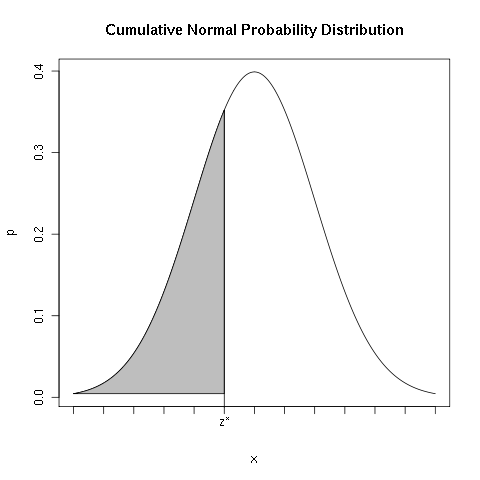
\includegraphics[height=2.25cm]{img/cummulativeDist}

\begin{tabular}{l|llllllllll}
     & 0.00   & 0.01   & 0.02   & 0.03   & 0.04   & 0.05   & 0.06   & 0.07   & 0.08  & 0.09 \\ \hline
-3.4 & 0.0003 & 0.0003 & 0.0003 & 0.0003 & 0.0003 & 0.0003 & 0.0003 & 0.0003 & 0.0003 & 0.0002 \\\arrayrulecolor{light-gray}\hline\arrayrulecolor{black} 
-3.3 & 0.0005 & 0.0005 & 0.0005 & 0.0004 & 0.0004 & 0.0004 & 0.0004 & 0.0004 & 0.0004 & 0.0003 \\\arrayrulecolor{light-gray}\hline\arrayrulecolor{black} 
-3.2 & 0.0007 & 0.0007 & 0.0006 & 0.0006 & 0.0006 & 0.0006 & 0.0006 & 0.0005 & 0.0005 & 0.0005 \\\arrayrulecolor{light-gray}\hline\arrayrulecolor{black} 
-3.1 & 0.0010 & 0.0009 & 0.0009 & 0.0009 & 0.0008 & 0.0008 & 0.0008 & 0.0008 & 0.0007 & 0.0007 \\\arrayrulecolor{light-gray}\hline\arrayrulecolor{black} 
-3.0 & 0.0013 & 0.0013 & 0.0013 & 0.0012 & 0.0012 & 0.0011 & 0.0011 & 0.0011 & 0.0010 & 0.0010 \\\arrayrulecolor{light-gray}\hline\arrayrulecolor{black} 
-2.9 & 0.0019 & 0.0018 & 0.0018 & 0.0017 & 0.0016 & 0.0016 & 0.0015 & 0.0015 & 0.0014 & 0.0014 \\\arrayrulecolor{light-gray}\hline\arrayrulecolor{black} 
-2.8 & 0.0026 & 0.0025 & 0.0024 & 0.0023 & 0.0023 & 0.0022 & 0.0021 & 0.0021 & 0.0020 & 0.0019 \\\arrayrulecolor{light-gray}\hline\arrayrulecolor{black} 
-2.7 & 0.0035 & 0.0034 & 0.0033 & 0.0032 & 0.0031 & 0.0030 & 0.0029 & 0.0028 & 0.0027 & 0.0026 \\\arrayrulecolor{light-gray}\hline\arrayrulecolor{black} 
-2.6 & 0.0047 & 0.0045 & 0.0044 & 0.0043 & 0.0041 & 0.0040 & 0.0039 & 0.0038 & 0.0037 & 0.0036 \\\arrayrulecolor{light-gray}\hline\arrayrulecolor{black} 
-2.5 & 0.0062 & 0.0060 & 0.0059 & 0.0057 & 0.0055 & 0.0054 & 0.0052 & 0.0051 & 0.0049 & 0.0048 \\\arrayrulecolor{light-gray}\hline\arrayrulecolor{black} 
-2.4 & 0.0082 & 0.0080 & 0.0078 & 0.0075 & 0.0073 & 0.0071 & 0.0069 & 0.0068 & 0.0066 & 0.0064 \\\arrayrulecolor{light-gray}\hline\arrayrulecolor{black} 
-2.3 & 0.0107 & 0.0104 & 0.0102 & 0.0099 & 0.0096 & 0.0094 & 0.0091 & 0.0089 & 0.0087 & 0.0084 \\\arrayrulecolor{light-gray}\hline\arrayrulecolor{black} 
-2.2 & 0.0139 & 0.0136 & 0.0132 & 0.0129 & 0.0125 & 0.0122 & 0.0119 & 0.0116 & 0.0113 & 0.0110 \\\arrayrulecolor{light-gray}\hline\arrayrulecolor{black} 
-2.1 & 0.0179 & 0.0174 & 0.0170 & 0.0166 & 0.0162 & 0.0158 & 0.0154 & 0.0150 & 0.0146 & 0.0143 \\\arrayrulecolor{light-gray}\hline\arrayrulecolor{black} 
-2.0 & 0.0228 & 0.0222 & 0.0217 & 0.0212 & 0.0207 & 0.0202 & 0.0197 & 0.0192 & 0.0188 & 0.0183 \\\arrayrulecolor{light-gray}\hline\arrayrulecolor{black} 
-1.9 & 0.0287 & 0.0281 & 0.0274 & 0.0268 & 0.0262 & 0.0256 & 0.0250 & 0.0244 & 0.0239 & 0.0233 \\\arrayrulecolor{light-gray}\hline\arrayrulecolor{black} 
-1.8 & 0.0359 & 0.0351 & 0.0344 & 0.0336 & 0.0329 & 0.0322 & 0.0314 & 0.0307 & 0.0301 & 0.0294 \\\arrayrulecolor{light-gray}\hline\arrayrulecolor{black} 
-1.7 & 0.0446 & 0.0436 & 0.0427 & 0.0418 & 0.0409 & 0.0401 & 0.0392 & 0.0384 & 0.0375 & 0.0367 \\\arrayrulecolor{light-gray}\hline\arrayrulecolor{black} 
-1.6 & 0.0548 & 0.0537 & 0.0526 & 0.0516 & 0.0505 & 0.0495 & 0.0485 & 0.0475 & 0.0465 & 0.0455 \\\arrayrulecolor{light-gray}\hline\arrayrulecolor{black} 
-1.5 & 0.0668 & 0.0655 & 0.0643 & 0.0630 & 0.0618 & 0.0606 & 0.0594 & 0.0582 & 0.0571 & 0.0559 \\\arrayrulecolor{light-gray}\hline\arrayrulecolor{black} 
-1.4 & 0.0808 & 0.0793 & 0.0778 & 0.0764 & 0.0749 & 0.0735 & 0.0721 & 0.0708 & 0.0694 & 0.0681 \\\arrayrulecolor{light-gray}\hline\arrayrulecolor{black} 
-1.3 & 0.0968 & 0.0951 & 0.0934 & 0.0918 & 0.0901 & 0.0885 & 0.0869 & 0.0853 & 0.0838 & 0.0823 \\\arrayrulecolor{light-gray}\hline\arrayrulecolor{black} 
-1.2 & 0.1151 & 0.1131 & 0.1112 & 0.1093 & 0.1075 & 0.1056 & 0.1038 & 0.1020 & 0.1003 & 0.0985 \\\arrayrulecolor{light-gray}\hline\arrayrulecolor{black} 
-1.1 & 0.1357 & 0.1335 & 0.1314 & 0.1292 & 0.1271 & 0.1251 & 0.1230 & 0.1210 & 0.1190 & 0.1170 \\\arrayrulecolor{light-gray}\hline\arrayrulecolor{black} 
-1.0 & 0.1587 & 0.1562 & 0.1539 & 0.1515 & 0.1492 & 0.1469 & 0.1446 & 0.1423 & 0.1401 & 0.1379 \\\arrayrulecolor{light-gray}\hline\arrayrulecolor{black} 
-0.9 & 0.1841 & 0.1814 & 0.1788 & 0.1762 & 0.1736 & 0.1711 & 0.1685 & 0.1660 & 0.1635 & 0.1611 \\\arrayrulecolor{light-gray}\hline\arrayrulecolor{black} 
-0.8 & 0.2119 & 0.2090 & 0.2061 & 0.2033 & 0.2005 & 0.1977 & 0.1949 & 0.1922 & 0.1894 & 0.1867 \\\arrayrulecolor{light-gray}\hline\arrayrulecolor{black} 
-0.7 & 0.2420 & 0.2389 & 0.2358 & 0.2327 & 0.2296 & 0.2266 & 0.2236 & 0.2206 & 0.2177 & 0.2148 \\\arrayrulecolor{light-gray}\hline\arrayrulecolor{black} 
-0.6 & 0.2743 & 0.2709 & 0.2676 & 0.2643 & 0.2611 & 0.2578 & 0.2546 & 0.2514 & 0.2483 & 0.2451 \\\arrayrulecolor{light-gray}\hline\arrayrulecolor{black} 
-0.5 & 0.3085 & 0.3050 & 0.3015 & 0.2981 & 0.2946 & 0.2912 & 0.2877 & 0.2843 & 0.2810 & 0.2776 \\\arrayrulecolor{light-gray}\hline\arrayrulecolor{black} 
-0.4 & 0.3446 & 0.3409 & 0.3372 & 0.3336 & 0.3300 & 0.3264 & 0.3228 & 0.3192 & 0.3156 & 0.3121 \\\arrayrulecolor{light-gray}\hline\arrayrulecolor{black} 
-0.3 & 0.3821 & 0.3783 & 0.3745 & 0.3707 & 0.3669 & 0.3632 & 0.3594 & 0.3557 & 0.3520 & 0.3483 \\\arrayrulecolor{light-gray}\hline\arrayrulecolor{black} 
-0.2 & 0.4207 & 0.4168 & 0.4129 & 0.4090 & 0.4052 & 0.4013 & 0.3974 & 0.3936 & 0.3897 & 0.3859 \\\arrayrulecolor{light-gray}\hline\arrayrulecolor{black} 
-0.1 & 0.4602 & 0.4562 & 0.4522 & 0.4483 & 0.4443 & 0.4404 & 0.4364 & 0.4325 & 0.4286 & 0.4247 \\\arrayrulecolor{light-gray}\hline\arrayrulecolor{black} 
-0.0 & 0.5000 & 0.4960 & 0.4920 & 0.4880 & 0.4840 & 0.4801 & 0.4761 & 0.4721 & 0.4681 & 0.4641 \\\arrayrulecolor{light-gray}\hline\arrayrulecolor{black} 
\end{tabular}


\clearpage
 Approximation of the cumulative distribution for the standard normal distribution. 
 \hfill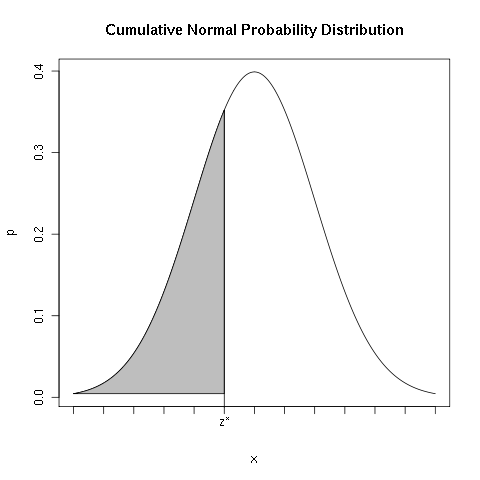
\includegraphics[height=3.25cm]{img/cummulativeDist}

 \begin{tabular}{l|llllllllll}
     & 0.00   & 0.01   & 0.02   & 0.03   & 0.04   & 0.05   & 0.06   & 0.07   & 0.08  & 0.09 \\ \hline
0.0 & 0.5000 & 0.5040 & 0.5080 & 0.5120 & 0.5160 & 0.5199 & 0.5239 & 0.5279 & 0.5319 & 0.5359 \\\arrayrulecolor{light-gray}\hline\arrayrulecolor{black} 
0.1 & 0.5398 & 0.5438 & 0.5478 & 0.5517 & 0.5557 & 0.5596 & 0.5636 & 0.5675 & 0.5714 & 0.5753 \\\arrayrulecolor{light-gray}\hline\arrayrulecolor{black} 
0.2 & 0.5793 & 0.5832 & 0.5871 & 0.5910 & 0.5948 & 0.5987 & 0.6026 & 0.6064 & 0.6103 & 0.6141 \\\arrayrulecolor{light-gray}\hline\arrayrulecolor{black} 
0.3 & 0.6179 & 0.6217 & 0.6255 & 0.6293 & 0.6331 & 0.6368 & 0.6406 & 0.6443 & 0.6480 & 0.6517 \\\arrayrulecolor{light-gray}\hline\arrayrulecolor{black} 
0.4 & 0.6554 & 0.6591 & 0.6628 & 0.6664 & 0.6700 & 0.6736 & 0.6772 & 0.6808 & 0.6844 & 0.6879 \\\arrayrulecolor{light-gray}\hline\arrayrulecolor{black} 
0.5 & 0.6915 & 0.6950 & 0.6985 & 0.7019 & 0.7054 & 0.7088 & 0.7123 & 0.7157 & 0.7190 & 0.7224 \\\arrayrulecolor{light-gray}\hline\arrayrulecolor{black} 
0.6 & 0.7257 & 0.7291 & 0.7324 & 0.7357 & 0.7389 & 0.7422 & 0.7454 & 0.7486 & 0.7517 & 0.7549 \\\arrayrulecolor{light-gray}\hline\arrayrulecolor{black} 
0.7 & 0.7580 & 0.7611 & 0.7642 & 0.7673 & 0.7704 & 0.7734 & 0.7764 & 0.7794 & 0.7823 & 0.7852 \\\arrayrulecolor{light-gray}\hline\arrayrulecolor{black} 
0.8 & 0.7881 & 0.7910 & 0.7939 & 0.7967 & 0.7995 & 0.8023 & 0.8051 & 0.8078 & 0.8106 & 0.8133 \\\arrayrulecolor{light-gray}\hline\arrayrulecolor{black} 
0.9 & 0.8159 & 0.8186 & 0.8212 & 0.8238 & 0.8264 & 0.8289 & 0.8315 & 0.8340 & 0.8365 & 0.8389 \\\arrayrulecolor{light-gray}\hline\arrayrulecolor{black} 
1.0 & 0.8413 & 0.8438 & 0.8461 & 0.8485 & 0.8508 & 0.8531 & 0.8554 & 0.8577 & 0.8599 & 0.8621 \\\arrayrulecolor{light-gray}\hline\arrayrulecolor{black} 
1.1 & 0.8643 & 0.8665 & 0.8686 & 0.8708 & 0.8729 & 0.8749 & 0.8770 & 0.8790 & 0.8810 & 0.8830 \\\arrayrulecolor{light-gray}\hline\arrayrulecolor{black} 
1.2 & 0.8849 & 0.8869 & 0.8888 & 0.8907 & 0.8925 & 0.8944 & 0.8962 & 0.8980 & 0.8997 & 0.9015 \\\arrayrulecolor{light-gray}\hline\arrayrulecolor{black} 
1.3 & 0.9032 & 0.9049 & 0.9066 & 0.9082 & 0.9099 & 0.9115 & 0.9131 & 0.9147 & 0.9162 & 0.9177 \\\arrayrulecolor{light-gray}\hline\arrayrulecolor{black} 
1.4 & 0.9192 & 0.9207 & 0.9222 & 0.9236 & 0.9251 & 0.9265 & 0.9279 & 0.9292 & 0.9306 & 0.9319 \\\arrayrulecolor{light-gray}\hline\arrayrulecolor{black} 
1.5 & 0.9332 & 0.9345 & 0.9357 & 0.9370 & 0.9382 & 0.9394 & 0.9406 & 0.9418 & 0.9429 & 0.9441 \\\arrayrulecolor{light-gray}\hline\arrayrulecolor{black} 
1.6 & 0.9452 & 0.9463 & 0.9474 & 0.9484 & 0.9495 & 0.9505 & 0.9515 & 0.9525 & 0.9535 & 0.9545 \\\arrayrulecolor{light-gray}\hline\arrayrulecolor{black} 
1.7 & 0.9554 & 0.9564 & 0.9573 & 0.9582 & 0.9591 & 0.9599 & 0.9608 & 0.9616 & 0.9625 & 0.9633 \\\arrayrulecolor{light-gray}\hline\arrayrulecolor{black} 
1.8 & 0.9641 & 0.9649 & 0.9656 & 0.9664 & 0.9671 & 0.9678 & 0.9686 & 0.9693 & 0.9699 & 0.9706 \\\arrayrulecolor{light-gray}\hline\arrayrulecolor{black} 
1.9 & 0.9713 & 0.9719 & 0.9726 & 0.9732 & 0.9738 & 0.9744 & 0.9750 & 0.9756 & 0.9761 & 0.9767 \\\arrayrulecolor{light-gray}\hline\arrayrulecolor{black} 
2.0 & 0.9772 & 0.9778 & 0.9783 & 0.9788 & 0.9793 & 0.9798 & 0.9803 & 0.9808 & 0.9812 & 0.9817 \\\arrayrulecolor{light-gray}\hline\arrayrulecolor{black} 
2.1 & 0.9821 & 0.9826 & 0.9830 & 0.9834 & 0.9838 & 0.9842 & 0.9846 & 0.9850 & 0.9854 & 0.9857 \\\arrayrulecolor{light-gray}\hline\arrayrulecolor{black} 
2.2 & 0.9861 & 0.9864 & 0.9868 & 0.9871 & 0.9875 & 0.9878 & 0.9881 & 0.9884 & 0.9887 & 0.9890 \\\arrayrulecolor{light-gray}\hline\arrayrulecolor{black} 
2.3 & 0.9893 & 0.9896 & 0.9898 & 0.9901 & 0.9904 & 0.9906 & 0.9909 & 0.9911 & 0.9913 & 0.9916 \\\arrayrulecolor{light-gray}\hline\arrayrulecolor{black} 
2.4 & 0.9918 & 0.9920 & 0.9922 & 0.9925 & 0.9927 & 0.9929 & 0.9931 & 0.9932 & 0.9934 & 0.9936 \\\arrayrulecolor{light-gray}\hline\arrayrulecolor{black} 
2.5 & 0.9938 & 0.9940 & 0.9941 & 0.9943 & 0.9945 & 0.9946 & 0.9948 & 0.9949 & 0.9951 & 0.9952 \\\arrayrulecolor{light-gray}\hline\arrayrulecolor{black} 
2.6 & 0.9953 & 0.9955 & 0.9956 & 0.9957 & 0.9959 & 0.9960 & 0.9961 & 0.9962 & 0.9963 & 0.9964 \\\arrayrulecolor{light-gray}\hline\arrayrulecolor{black} 
2.7 & 0.9965 & 0.9966 & 0.9967 & 0.9968 & 0.9969 & 0.9970 & 0.9971 & 0.9972 & 0.9973 & 0.9974 \\\arrayrulecolor{light-gray}\hline\arrayrulecolor{black} 
2.8 & 0.9974 & 0.9975 & 0.9976 & 0.9977 & 0.9977 & 0.9978 & 0.9979 & 0.9979 & 0.9980 & 0.9981 \\\arrayrulecolor{light-gray}\hline\arrayrulecolor{black} 
2.9 & 0.9981 & 0.9982 & 0.9982 & 0.9983 & 0.9984 & 0.9984 & 0.9985 & 0.9985 & 0.9986 & 0.9986 \\\arrayrulecolor{light-gray}\hline\arrayrulecolor{black} 
3.0 & 0.9987 & 0.9987 & 0.9987 & 0.9988 & 0.9988 & 0.9989 & 0.9989 & 0.9989 & 0.9990 & 0.9990 \\\arrayrulecolor{light-gray}\hline\arrayrulecolor{black} 
3.1 & 0.9990 & 0.9991 & 0.9991 & 0.9991 & 0.9992 & 0.9992 & 0.9992 & 0.9992 & 0.9993 & 0.9993 \\\arrayrulecolor{light-gray}\hline\arrayrulecolor{black} 
3.2 & 0.9993 & 0.9993 & 0.9994 & 0.9994 & 0.9994 & 0.9994 & 0.9994 & 0.9995 & 0.9995 & 0.9995 \\\arrayrulecolor{light-gray}\hline\arrayrulecolor{black} 
3.3 & 0.9995 & 0.9995 & 0.9995 & 0.9996 & 0.9996 & 0.9996 & 0.9996 & 0.9996 & 0.9996 & 0.9997 \\\arrayrulecolor{light-gray}\hline\arrayrulecolor{black} 
3.4 & 0.9997 & 0.9997 & 0.9997 & 0.9997 & 0.9997 & 0.9997 & 0.9997 & 0.9997 & 0.9997 & 0.9998 \\\arrayrulecolor{light-gray}\hline\arrayrulecolor{black} 
\end{tabular}

\clearpage

\section{Critical t tables}

 Approximation of the critical values for the $t$-distribution. 

 \hfill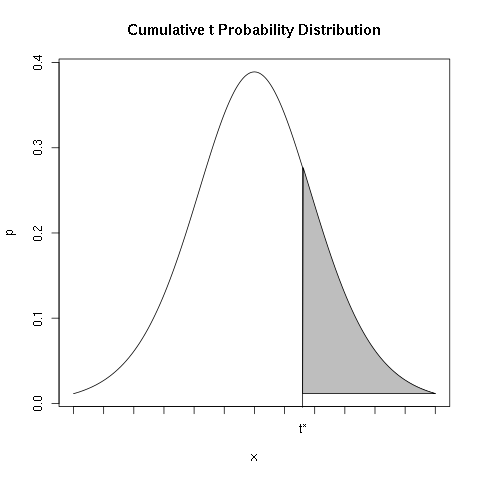
\includegraphics[height=3.0cm]{img/tcummulativeDist}

 \rowcolors{2}{gray!15}{white}
{
 \fontencoding{T1}
 \fontfamily{pcr}
 \fontseries{m}
 \fontshape{n}
 \fontsize{6pt}{6pt}
 \selectfont
\begin{tabular}{m{6pt}|m{24pt}*{11}{m{24pt}}}\hline 
df  & p=0.25 & 0.2000 & 0.1500 & 0.1000 & 0.0500 & 0.0250 & 0.0200 & 0.0100 & 0.0050 & 0.0025 & 0.0010 & 0.0005 \\\hline 
  1 & 1.0000 & 1.3764 & 1.9626 & 3.0777 & 6.3138 & 12.7062 & 15.8945 & 31.8205 & 63.6567 & 127.3213 & 318.3088 & 636.6192 \\[1pt] \arrayrulecolor{light-gray}\hline\arrayrulecolor{black}  
  2 & 0.8165 & 1.0607 & 1.3862 & 1.8856 & 2.9200 & 4.3027 & 4.8487 & 6.9646 & 9.9248 & 14.0890 & 22.3271 & 31.5991 \\[1pt] \arrayrulecolor{light-gray}\hline\arrayrulecolor{black}  
  3 & 0.7649 & 0.9785 & 1.2498 & 1.6377 & 2.3534 & 3.1824 & 3.4819 & 4.5407 & 5.8409 & 7.4533 & 10.2145 & 12.9240 \\[1pt] \arrayrulecolor{light-gray}\hline\arrayrulecolor{black}  
  4 & 0.7407 & 0.9410 & 1.1896 & 1.5332 & 2.1318 & 2.7764 & 2.9985 & 3.7469 & 4.6041 & 5.5976 & 7.1732 & 8.6103 \\[1pt] \arrayrulecolor{light-gray}\hline\arrayrulecolor{black}  
  5 & 0.7267 & 0.9195 & 1.1558 & 1.4759 & 2.0150 & 2.5706 & 2.7565 & 3.3649 & 4.0321 & 4.7733 & 5.8934 & 6.8688 \\[1pt] \arrayrulecolor{light-gray}\hline\arrayrulecolor{black}  
  6 & 0.7176 & 0.9057 & 1.1342 & 1.4398 & 1.9432 & 2.4469 & 2.6122 & 3.1427 & 3.7074 & 4.3168 & 5.2076 & 5.9588 \\[1pt] \arrayrulecolor{light-gray}\hline\arrayrulecolor{black}  
  7 & 0.7111 & 0.8960 & 1.1192 & 1.4149 & 1.8946 & 2.3646 & 2.5168 & 2.9980 & 3.4995 & 4.0293 & 4.7853 & 5.4079 \\[1pt] \arrayrulecolor{light-gray}\hline\arrayrulecolor{black}  
  8 & 0.7064 & 0.8889 & 1.1081 & 1.3968 & 1.8595 & 2.3060 & 2.4490 & 2.8965 & 3.3554 & 3.8325 & 4.5008 & 5.0413 \\[1pt] \arrayrulecolor{light-gray}\hline\arrayrulecolor{black}  
  9 & 0.7027 & 0.8834 & 1.0997 & 1.3830 & 1.8331 & 2.2622 & 2.3984 & 2.8214 & 3.2498 & 3.6897 & 4.2968 & 4.7809 \\[1pt] \arrayrulecolor{light-gray}\hline\arrayrulecolor{black}  
 10 & 0.6998 & 0.8791 & 1.0931 & 1.3722 & 1.8125 & 2.2281 & 2.3593 & 2.7638 & 3.1693 & 3.5814 & 4.1437 & 4.5869 \\[1pt] \arrayrulecolor{light-gray}\hline\arrayrulecolor{black}  
 11 & 0.6974 & 0.8755 & 1.0877 & 1.3634 & 1.7959 & 2.2010 & 2.3281 & 2.7181 & 3.1058 & 3.4966 & 4.0247 & 4.4370 \\[1pt] \arrayrulecolor{light-gray}\hline\arrayrulecolor{black}  
 12 & 0.6955 & 0.8726 & 1.0832 & 1.3562 & 1.7823 & 2.1788 & 2.3027 & 2.6810 & 3.0545 & 3.4284 & 3.9296 & 4.3178 \\[1pt] \arrayrulecolor{light-gray}\hline\arrayrulecolor{black}  
 13 & 0.6938 & 0.8702 & 1.0795 & 1.3502 & 1.7709 & 2.1604 & 2.2816 & 2.6503 & 3.0123 & 3.3725 & 3.8520 & 4.2208 \\[1pt] \arrayrulecolor{light-gray}\hline\arrayrulecolor{black}  
 14 & 0.6924 & 0.8681 & 1.0763 & 1.3450 & 1.7613 & 2.1448 & 2.2638 & 2.6245 & 2.9768 & 3.3257 & 3.7874 & 4.1405 \\[1pt] \arrayrulecolor{light-gray}\hline\arrayrulecolor{black}  
 15 & 0.6912 & 0.8662 & 1.0735 & 1.3406 & 1.7531 & 2.1314 & 2.2485 & 2.6025 & 2.9467 & 3.2860 & 3.7328 & 4.0728 \\[1pt] \arrayrulecolor{light-gray}\hline\arrayrulecolor{black}  
 16 & 0.6901 & 0.8647 & 1.0711 & 1.3368 & 1.7459 & 2.1199 & 2.2354 & 2.5835 & 2.9208 & 3.2520 & 3.6862 & 4.0150 \\[1pt] \arrayrulecolor{light-gray}\hline\arrayrulecolor{black}  
 17 & 0.6892 & 0.8633 & 1.0690 & 1.3334 & 1.7396 & 2.1098 & 2.2238 & 2.5669 & 2.8982 & 3.2224 & 3.6458 & 3.9651 \\[1pt] \arrayrulecolor{light-gray}\hline\arrayrulecolor{black}  
 18 & 0.6884 & 0.8620 & 1.0672 & 1.3304 & 1.7341 & 2.1009 & 2.2137 & 2.5524 & 2.8784 & 3.1966 & 3.6105 & 3.9216 \\[1pt] \arrayrulecolor{light-gray}\hline\arrayrulecolor{black}  
 19 & 0.6876 & 0.8610 & 1.0655 & 1.3277 & 1.7291 & 2.0930 & 2.2047 & 2.5395 & 2.8609 & 3.1737 & 3.5794 & 3.8834 \\[1pt] \arrayrulecolor{light-gray}\hline\arrayrulecolor{black}  
 20 & 0.6870 & 0.8600 & 1.0640 & 1.3253 & 1.7247 & 2.0860 & 2.1967 & 2.5280 & 2.8453 & 3.1534 & 3.5518 & 3.8495 \\[1pt] \arrayrulecolor{light-gray}\hline\arrayrulecolor{black}  
 21 & 0.6864 & 0.8591 & 1.0627 & 1.3232 & 1.7207 & 2.0796 & 2.1894 & 2.5176 & 2.8314 & 3.1352 & 3.5272 & 3.8193 \\[1pt] \arrayrulecolor{light-gray}\hline\arrayrulecolor{black}  
 22 & 0.6858 & 0.8583 & 1.0614 & 1.3212 & 1.7171 & 2.0739 & 2.1829 & 2.5083 & 2.8188 & 3.1188 & 3.5050 & 3.7921 \\[1pt] \arrayrulecolor{light-gray}\hline\arrayrulecolor{black}  
 23 & 0.6853 & 0.8575 & 1.0603 & 1.3195 & 1.7139 & 2.0687 & 2.1770 & 2.4999 & 2.8073 & 3.1040 & 3.4850 & 3.7676 \\[1pt] \arrayrulecolor{light-gray}\hline\arrayrulecolor{black}  
 24 & 0.6848 & 0.8569 & 1.0593 & 1.3178 & 1.7109 & 2.0639 & 2.1715 & 2.4922 & 2.7969 & 3.0905 & 3.4668 & 3.7454 \\[1pt] \arrayrulecolor{light-gray}\hline\arrayrulecolor{black}  
 25 & 0.6844 & 0.8562 & 1.0584 & 1.3163 & 1.7081 & 2.0595 & 2.1666 & 2.4851 & 2.7874 & 3.0782 & 3.4502 & 3.7251 \\[1pt] \arrayrulecolor{light-gray}\hline\arrayrulecolor{black}  
 26 & 0.6840 & 0.8557 & 1.0575 & 1.3150 & 1.7056 & 2.0555 & 2.1620 & 2.4786 & 2.7787 & 3.0669 & 3.4350 & 3.7066 \\[1pt] \arrayrulecolor{light-gray}\hline\arrayrulecolor{black}  
 27 & 0.6837 & 0.8551 & 1.0567 & 1.3137 & 1.7033 & 2.0518 & 2.1578 & 2.4727 & 2.7707 & 3.0565 & 3.4210 & 3.6896 \\[1pt] \arrayrulecolor{light-gray}\hline\arrayrulecolor{black}  
 28 & 0.6834 & 0.8546 & 1.0560 & 1.3125 & 1.7011 & 2.0484 & 2.1539 & 2.4671 & 2.7633 & 3.0469 & 3.4082 & 3.6739 \\[1pt] \arrayrulecolor{light-gray}\hline\arrayrulecolor{black}  
 29 & 0.6830 & 0.8542 & 1.0553 & 1.3114 & 1.6991 & 2.0452 & 2.1503 & 2.4620 & 2.7564 & 3.0380 & 3.3962 & 3.6594 \\[1pt] \arrayrulecolor{light-gray}\hline\arrayrulecolor{black}  
 30 & 0.6828 & 0.8538 & 1.0547 & 1.3104 & 1.6973 & 2.0423 & 2.1470 & 2.4573 & 2.7500 & 3.0298 & 3.3852 & 3.6460 \\[1pt] \arrayrulecolor{light-gray}\hline\arrayrulecolor{black}  
 31 & 0.6825 & 0.8534 & 1.0541 & 1.3095 & 1.6955 & 2.0395 & 2.1438 & 2.4528 & 2.7440 & 3.0221 & 3.3749 & 3.6335 \\[1pt] \arrayrulecolor{light-gray}\hline\arrayrulecolor{black}  
 32 & 0.6822 & 0.8530 & 1.0535 & 1.3086 & 1.6939 & 2.0369 & 2.1409 & 2.4487 & 2.7385 & 3.0149 & 3.3653 & 3.6218 \\[1pt] \arrayrulecolor{light-gray}\hline\arrayrulecolor{black}  
 33 & 0.6820 & 0.8526 & 1.0530 & 1.3077 & 1.6924 & 2.0345 & 2.1382 & 2.4448 & 2.7333 & 3.0082 & 3.3563 & 3.6109 \\[1pt] \arrayrulecolor{light-gray}\hline\arrayrulecolor{black}  
 34 & 0.6818 & 0.8523 & 1.0525 & 1.3070 & 1.6909 & 2.0322 & 2.1356 & 2.4411 & 2.7284 & 3.0020 & 3.3479 & 3.6007 \\[1pt] \arrayrulecolor{light-gray}\hline\arrayrulecolor{black}  
 35 & 0.6816 & 0.8520 & 1.0520 & 1.3062 & 1.6896 & 2.0301 & 2.1332 & 2.4377 & 2.7238 & 2.9960 & 3.3400 & 3.5911 \\[1pt] \arrayrulecolor{light-gray}\hline\arrayrulecolor{black}  
 36 & 0.6814 & 0.8517 & 1.0516 & 1.3055 & 1.6883 & 2.0281 & 2.1309 & 2.4345 & 2.7195 & 2.9905 & 3.3326 & 3.5821 \\[1pt] \arrayrulecolor{light-gray}\hline\arrayrulecolor{black}  
 37 & 0.6812 & 0.8514 & 1.0512 & 1.3049 & 1.6871 & 2.0262 & 2.1287 & 2.4314 & 2.7154 & 2.9852 & 3.3256 & 3.5737 \\[1pt] \arrayrulecolor{light-gray}\hline\arrayrulecolor{black}  
 38 & 0.6810 & 0.8512 & 1.0508 & 1.3042 & 1.6860 & 2.0244 & 2.1267 & 2.4286 & 2.7116 & 2.9803 & 3.3190 & 3.5657 \\[1pt] \arrayrulecolor{light-gray}\hline\arrayrulecolor{black}  
 39 & 0.6808 & 0.8509 & 1.0504 & 1.3036 & 1.6849 & 2.0227 & 2.1247 & 2.4258 & 2.7079 & 2.9756 & 3.3128 & 3.5581 \\[1pt] \arrayrulecolor{light-gray}\hline\arrayrulecolor{black}  
 40 & 0.6807 & 0.8507 & 1.0500 & 1.3031 & 1.6839 & 2.0211 & 2.1229 & 2.4233 & 2.7045 & 2.9712 & 3.3069 & 3.5510 \\[1pt] \arrayrulecolor{light-gray}\hline\arrayrulecolor{black}  
 41 & 0.6805 & 0.8505 & 1.0497 & 1.3025 & 1.6829 & 2.0195 & 2.1212 & 2.4208 & 2.7012 & 2.9670 & 3.3013 & 3.5442 \\[1pt] \arrayrulecolor{light-gray}\hline\arrayrulecolor{black}  
 42 & 0.6804 & 0.8503 & 1.0494 & 1.3020 & 1.6820 & 2.0181 & 2.1195 & 2.4185 & 2.6981 & 2.9630 & 3.2960 & 3.5377 \\[1pt] \arrayrulecolor{light-gray}\hline\arrayrulecolor{black}  
 43 & 0.6802 & 0.8501 & 1.0491 & 1.3016 & 1.6811 & 2.0167 & 2.1179 & 2.4163 & 2.6951 & 2.9592 & 3.2909 & 3.5316 \\[1pt] \arrayrulecolor{light-gray}\hline\arrayrulecolor{black}  
 44 & 0.6801 & 0.8499 & 1.0488 & 1.3011 & 1.6802 & 2.0154 & 2.1164 & 2.4141 & 2.6923 & 2.9555 & 3.2861 & 3.5258 \\[1pt] \arrayrulecolor{light-gray}\hline\arrayrulecolor{black}  
 45 & 0.6800 & 0.8497 & 1.0485 & 1.3006 & 1.6794 & 2.0141 & 2.1150 & 2.4121 & 2.6896 & 2.9521 & 3.2815 & 3.5203 \\[1pt] \arrayrulecolor{light-gray}\hline\arrayrulecolor{black}  
 46 & 0.6799 & 0.8495 & 1.0483 & 1.3002 & 1.6787 & 2.0129 & 2.1136 & 2.4102 & 2.6870 & 2.9488 & 3.2771 & 3.5150 \\[1pt] \arrayrulecolor{light-gray}\hline\arrayrulecolor{black}  
 47 & 0.6797 & 0.8493 & 1.0480 & 1.2998 & 1.6779 & 2.0117 & 2.1123 & 2.4083 & 2.6846 & 2.9456 & 3.2729 & 3.5099 \\[1pt] \arrayrulecolor{light-gray}\hline\arrayrulecolor{black}  
 48 & 0.6796 & 0.8492 & 1.0478 & 1.2994 & 1.6772 & 2.0106 & 2.1111 & 2.4066 & 2.6822 & 2.9426 & 3.2689 & 3.5051 \\[1pt] \arrayrulecolor{light-gray}\hline\arrayrulecolor{black}  
 49 & 0.6795 & 0.8490 & 1.0475 & 1.2991 & 1.6766 & 2.0096 & 2.1099 & 2.4049 & 2.6800 & 2.9397 & 3.2651 & 3.5004 \\[1pt] \arrayrulecolor{light-gray}\hline\arrayrulecolor{black}  
 50 & 0.6794 & 0.8489 & 1.0473 & 1.2987 & 1.6759 & 2.0086 & 2.1087 & 2.4033 & 2.6778 & 2.9370 & 3.2614 & 3.4960 \\[1pt] \arrayrulecolor{light-gray}\hline\arrayrulecolor{black}  
 51 & 0.6793 & 0.8487 & 1.0471 & 1.2984 & 1.6753 & 2.0076 & 2.1076 & 2.4017 & 2.6757 & 2.9343 & 3.2579 & 3.4918 \\[1pt] \arrayrulecolor{light-gray}\hline\arrayrulecolor{black}  
 52 & 0.6792 & 0.8486 & 1.0469 & 1.2980 & 1.6747 & 2.0066 & 2.1066 & 2.4002 & 2.6737 & 2.9318 & 3.2545 & 3.4877 \\[1pt] \arrayrulecolor{light-gray}\hline\arrayrulecolor{black}  
 53 & 0.6791 & 0.8485 & 1.0467 & 1.2977 & 1.6741 & 2.0057 & 2.1055 & 2.3988 & 2.6718 & 2.9293 & 3.2513 & 3.4838 \\[1pt] \arrayrulecolor{light-gray}\hline\arrayrulecolor{black}  
 54 & 0.6791 & 0.8483 & 1.0465 & 1.2974 & 1.6736 & 2.0049 & 2.1046 & 2.3974 & 2.6700 & 2.9270 & 3.2481 & 3.4800 \\[1pt] \arrayrulecolor{light-gray}\hline\arrayrulecolor{black}  
 55 & 0.6790 & 0.8482 & 1.0463 & 1.2971 & 1.6730 & 2.0040 & 2.1036 & 2.3961 & 2.6682 & 2.9247 & 3.2451 & 3.4764 \\[1pt] \arrayrulecolor{light-gray}\hline\arrayrulecolor{black}  
 56 & 0.6789 & 0.8481 & 1.0461 & 1.2969 & 1.6725 & 2.0032 & 2.1027 & 2.3948 & 2.6665 & 2.9225 & 3.2423 & 3.4729 \\[1pt] \arrayrulecolor{light-gray}\hline\arrayrulecolor{black}  
 57 & 0.6788 & 0.8480 & 1.0459 & 1.2966 & 1.6720 & 2.0025 & 2.1018 & 2.3936 & 2.6649 & 2.9204 & 3.2395 & 3.4696 \\[1pt] \arrayrulecolor{light-gray}\hline\arrayrulecolor{black}  
 58 & 0.6787 & 0.8479 & 1.0458 & 1.2963 & 1.6716 & 2.0017 & 2.1010 & 2.3924 & 2.6633 & 2.9184 & 3.2368 & 3.4663 \\[1pt] \arrayrulecolor{light-gray}\hline\arrayrulecolor{black}  
 59 & 0.6787 & 0.8478 & 1.0456 & 1.2961 & 1.6711 & 2.0010 & 2.1002 & 2.3912 & 2.6618 & 2.9164 & 3.2342 & 3.4632 \\[1pt] \arrayrulecolor{light-gray}\hline\arrayrulecolor{black}  
 60 & 0.6786 & 0.8477 & 1.0455 & 1.2958 & 1.6706 & 2.0003 & 2.0994 & 2.3901 & 2.6603 & 2.9146 & 3.2317 & 3.4602 \\[1pt] \arrayrulecolor{light-gray}\hline\arrayrulecolor{black}  
 70 & 0.6780 & 0.8468 & 1.0442 & 1.2938 & 1.6669 & 1.9944 & 2.0927 & 2.3808 & 2.6479 & 2.8987 & 3.2108 & 3.4350 \\[1pt] \arrayrulecolor{light-gray}\hline\arrayrulecolor{black}  
 80 & 0.6776 & 0.8461 & 1.0432 & 1.2922 & 1.6641 & 1.9901 & 2.0878 & 2.3739 & 2.6387 & 2.8870 & 3.1953 & 3.4163 \\[1pt] \arrayrulecolor{light-gray}\hline\arrayrulecolor{black}  
 90 & 0.6772 & 0.8456 & 1.0424 & 1.2910 & 1.6620 & 1.9867 & 2.0839 & 2.3685 & 2.6316 & 2.8779 & 3.1833 & 3.4019 \\[1pt] \arrayrulecolor{light-gray}\hline\arrayrulecolor{black}  
100 & 0.6770 & 0.8452 & 1.0418 & 1.2901 & 1.6602 & 1.9840 & 2.0809 & 2.3642 & 2.6259 & 2.8707 & 3.1737 & 3.3905 \\[1pt] \arrayrulecolor{light-gray}\hline\arrayrulecolor{black}  
110 & 0.6767 & 0.8449 & 1.0413 & 1.2893 & 1.6588 & 1.9818 & 2.0784 & 2.3607 & 2.6213 & 2.8648 & 3.1660 & 3.3812 \\[1pt] \arrayrulecolor{light-gray}\hline\arrayrulecolor{black}  
120 & 0.6765 & 0.8446 & 1.0409 & 1.2886 & 1.6577 & 1.9799 & 2.0763 & 2.3578 & 2.6174 & 2.8599 & 3.1595 & 3.3735 \\[1pt] \arrayrulecolor{light-gray}\hline\arrayrulecolor{black}  
$\infty$  & 0.6745 & 0.8416 & 1.0364 & 1.2816 & 1.6449 & 1.9600 & 2.0537 & 2.3263 & 2.5758 & 2.8070 & 3.0902 & 3.2905 \\[5pt] \arrayrulecolor{light-gray}\hline\arrayrulecolor{black}  
\end{tabular}
}


\section{Critical F Tables}

Approximation of the critical values for the $F$-distribution for $\alpha=$ 0.1 . 
 %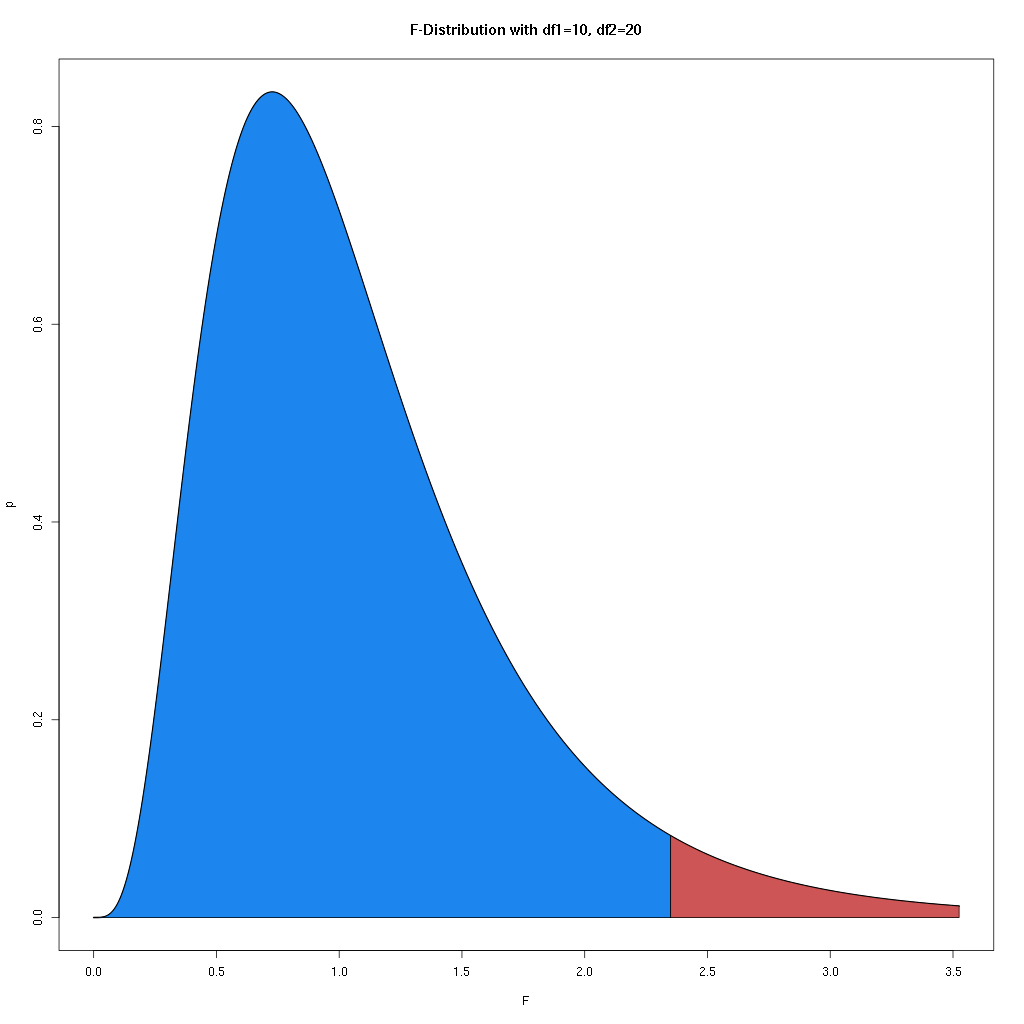
\includegraphics[height=2.0cm]{img/FDistribution}

 {\fontencoding{T1}
 \fontfamily{pcr}
 \fontseries{m}
 \fontshape{n}
 \fontsize{5pt}{5pt}
 \selectfont
\begin{tabular}{l|lllllllllllll} 
df2  & df1      1  &      2  &      3  &      4  &      5  &      6  &      7  &      8  &      9  &     10  &     12  &     15  &     20   \\ 
  1 & 39.8635 & 49.5000 & 53.5932 & 55.8330 & 57.2401 & 58.2044 & 58.9060 & 59.4390 & 59.8576 & 60.1950 & 60.7052 & 61.2203 & 61.7403 \\[5pt] \arrayrulecolor{light-gray}\hline\arrayrulecolor{black}  
  2 & 8.5263 & 9.0000 & 9.1618 & 9.2434 & 9.2926 & 9.3255 & 9.3491 & 9.3668 & 9.3805 & 9.3916 & 9.4081 & 9.4247 & 9.4413 \\[5pt] \arrayrulecolor{light-gray}\hline\arrayrulecolor{black}  
  3 & 5.5383 & 5.4624 & 5.3908 & 5.3426 & 5.3092 & 5.2847 & 5.2662 & 5.2517 & 5.2400 & 5.2304 & 5.2156 & 5.2003 & 5.1845 \\[5pt] \arrayrulecolor{light-gray}\hline\arrayrulecolor{black}  
  4 & 4.5448 & 4.3246 & 4.1909 & 4.1072 & 4.0506 & 4.0097 & 3.9790 & 3.9549 & 3.9357 & 3.9199 & 3.8955 & 3.8704 & 3.8443 \\[5pt] \arrayrulecolor{light-gray}\hline\arrayrulecolor{black}  
  5 & 4.0604 & 3.7797 & 3.6195 & 3.5202 & 3.4530 & 3.4045 & 3.3679 & 3.3393 & 3.3163 & 3.2974 & 3.2682 & 3.2380 & 3.2067 \\[5pt] \arrayrulecolor{light-gray}\hline\arrayrulecolor{black}  
\\ 
  6 & 3.7759 & 3.4633 & 3.2888 & 3.1808 & 3.1075 & 3.0546 & 3.0145 & 2.9830 & 2.9577 & 2.9369 & 2.9047 & 2.8712 & 2.8363 \\[5pt] \arrayrulecolor{light-gray}\hline\arrayrulecolor{black}  
  7 & 3.5894 & 3.2574 & 3.0741 & 2.9605 & 2.8833 & 2.8274 & 2.7849 & 2.7516 & 2.7247 & 2.7025 & 2.6681 & 2.6322 & 2.5947 \\[5pt] \arrayrulecolor{light-gray}\hline\arrayrulecolor{black}  
  8 & 3.4579 & 3.1131 & 2.9238 & 2.8064 & 2.7264 & 2.6683 & 2.6241 & 2.5893 & 2.5612 & 2.5380 & 2.5020 & 2.4642 & 2.4246 \\[5pt] \arrayrulecolor{light-gray}\hline\arrayrulecolor{black}  
  9 & 3.3603 & 3.0065 & 2.8129 & 2.6927 & 2.6106 & 2.5509 & 2.5053 & 2.4694 & 2.4403 & 2.4163 & 2.3789 & 2.3396 & 2.2983 \\[5pt] \arrayrulecolor{light-gray}\hline\arrayrulecolor{black}  
 10 & 3.2850 & 2.9245 & 2.7277 & 2.6053 & 2.5216 & 2.4606 & 2.4140 & 2.3772 & 2.3473 & 2.3226 & 2.2841 & 2.2435 & 2.2007 \\[5pt] \arrayrulecolor{light-gray}\hline\arrayrulecolor{black}  
\\ 
 11 & 3.2252 & 2.8595 & 2.6602 & 2.5362 & 2.4512 & 2.3891 & 2.3416 & 2.3040 & 2.2735 & 2.2482 & 2.2087 & 2.1671 & 2.1230 \\[5pt] \arrayrulecolor{light-gray}\hline\arrayrulecolor{black}  
 12 & 3.1765 & 2.8068 & 2.6055 & 2.4801 & 2.3940 & 2.3310 & 2.2828 & 2.2446 & 2.2135 & 2.1878 & 2.1474 & 2.1049 & 2.0597 \\[5pt] \arrayrulecolor{light-gray}\hline\arrayrulecolor{black}  
 13 & 3.1362 & 2.7632 & 2.5603 & 2.4337 & 2.3467 & 2.2830 & 2.2341 & 2.1953 & 2.1638 & 2.1376 & 2.0966 & 2.0532 & 2.0070 \\[5pt] \arrayrulecolor{light-gray}\hline\arrayrulecolor{black}  
 14 & 3.1022 & 2.7265 & 2.5222 & 2.3947 & 2.3069 & 2.2426 & 2.1931 & 2.1539 & 2.1220 & 2.0954 & 2.0537 & 2.0095 & 1.9625 \\[5pt] \arrayrulecolor{light-gray}\hline\arrayrulecolor{black}  
 15 & 3.0732 & 2.6952 & 2.4898 & 2.3614 & 2.2730 & 2.2081 & 2.1582 & 2.1185 & 2.0862 & 2.0593 & 2.0171 & 1.9722 & 1.9243 \\[5pt] \arrayrulecolor{light-gray}\hline\arrayrulecolor{black}  
\\ 
 16 & 3.0481 & 2.6682 & 2.4618 & 2.3327 & 2.2438 & 2.1783 & 2.1280 & 2.0880 & 2.0553 & 2.0281 & 1.9854 & 1.9399 & 1.8913 \\[5pt] \arrayrulecolor{light-gray}\hline\arrayrulecolor{black}  
 17 & 3.0262 & 2.6446 & 2.4374 & 2.3077 & 2.2183 & 2.1524 & 2.1017 & 2.0613 & 2.0284 & 2.0009 & 1.9577 & 1.9117 & 1.8624 \\[5pt] \arrayrulecolor{light-gray}\hline\arrayrulecolor{black}  
 18 & 3.0070 & 2.6239 & 2.4160 & 2.2858 & 2.1958 & 2.1296 & 2.0785 & 2.0379 & 2.0047 & 1.9770 & 1.9333 & 1.8868 & 1.8368 \\[5pt] \arrayrulecolor{light-gray}\hline\arrayrulecolor{black}  
 19 & 2.9899 & 2.6056 & 2.3970 & 2.2663 & 2.1760 & 2.1094 & 2.0580 & 2.0171 & 1.9836 & 1.9557 & 1.9117 & 1.8647 & 1.8142 \\[5pt] \arrayrulecolor{light-gray}\hline\arrayrulecolor{black}  
 20 & 2.9747 & 2.5893 & 2.3801 & 2.2489 & 2.1582 & 2.0913 & 2.0397 & 1.9985 & 1.9649 & 1.9367 & 1.8924 & 1.8449 & 1.7938 \\[5pt] \arrayrulecolor{light-gray}\hline\arrayrulecolor{black}  
\\ 
 21 & 2.9610 & 2.5746 & 2.3649 & 2.2333 & 2.1423 & 2.0751 & 2.0233 & 1.9819 & 1.9480 & 1.9197 & 1.8750 & 1.8271 & 1.7756 \\[5pt] \arrayrulecolor{light-gray}\hline\arrayrulecolor{black}  
 22 & 2.9486 & 2.5613 & 2.3512 & 2.2193 & 2.1279 & 2.0605 & 2.0084 & 1.9668 & 1.9327 & 1.9043 & 1.8593 & 1.8111 & 1.7590 \\[5pt] \arrayrulecolor{light-gray}\hline\arrayrulecolor{black}  
 23 & 2.9374 & 2.5493 & 2.3387 & 2.2065 & 2.1149 & 2.0472 & 1.9949 & 1.9531 & 1.9189 & 1.8903 & 1.8450 & 1.7964 & 1.7439 \\[5pt] \arrayrulecolor{light-gray}\hline\arrayrulecolor{black}  
 24 & 2.9271 & 2.5383 & 2.3274 & 2.1949 & 2.1030 & 2.0351 & 1.9826 & 1.9407 & 1.9063 & 1.8775 & 1.8319 & 1.7831 & 1.7302 \\[5pt] \arrayrulecolor{light-gray}\hline\arrayrulecolor{black}  
 25 & 2.9177 & 2.5283 & 2.3170 & 2.1842 & 2.0922 & 2.0241 & 1.9714 & 1.9292 & 1.8947 & 1.8658 & 1.8200 & 1.7708 & 1.7175 \\[5pt] \arrayrulecolor{light-gray}\hline\arrayrulecolor{black}  
\\ 
 26 & 2.9091 & 2.5191 & 2.3075 & 2.1745 & 2.0822 & 2.0139 & 1.9610 & 1.9188 & 1.8841 & 1.8550 & 1.8090 & 1.7596 & 1.7059 \\[5pt] \arrayrulecolor{light-gray}\hline\arrayrulecolor{black}  
 27 & 2.9012 & 2.5106 & 2.2987 & 2.1655 & 2.0730 & 2.0045 & 1.9515 & 1.9091 & 1.8743 & 1.8451 & 1.7989 & 1.7492 & 1.6951 \\[5pt] \arrayrulecolor{light-gray}\hline\arrayrulecolor{black}  
 28 & 2.8938 & 2.5028 & 2.2906 & 2.1571 & 2.0645 & 1.9959 & 1.9427 & 1.9001 & 1.8652 & 1.8359 & 1.7895 & 1.7395 & 1.6852 \\[5pt] \arrayrulecolor{light-gray}\hline\arrayrulecolor{black}  
 29 & 2.8870 & 2.4955 & 2.2831 & 2.1494 & 2.0566 & 1.9878 & 1.9345 & 1.8918 & 1.8568 & 1.8274 & 1.7808 & 1.7306 & 1.6759 \\[5pt] \arrayrulecolor{light-gray}\hline\arrayrulecolor{black}  
 30 & 2.8807 & 2.4887 & 2.2761 & 2.1422 & 2.0492 & 1.9803 & 1.9269 & 1.8841 & 1.8490 & 1.8195 & 1.7727 & 1.7223 & 1.6673 \\[5pt] \arrayrulecolor{light-gray}\hline\arrayrulecolor{black}  
\\ 
 31 & 2.8748 & 2.4824 & 2.2695 & 2.1355 & 2.0424 & 1.9734 & 1.9198 & 1.8769 & 1.8417 & 1.8121 & 1.7651 & 1.7145 & 1.6593 \\[5pt] \arrayrulecolor{light-gray}\hline\arrayrulecolor{black}  
 32 & 2.8693 & 2.4765 & 2.2635 & 2.1293 & 2.0360 & 1.9668 & 1.9132 & 1.8702 & 1.8348 & 1.8052 & 1.7581 & 1.7072 & 1.6517 \\[5pt] \arrayrulecolor{light-gray}\hline\arrayrulecolor{black}  
 33 & 2.8641 & 2.4710 & 2.2577 & 2.1234 & 2.0300 & 1.9607 & 1.9070 & 1.8639 & 1.8284 & 1.7987 & 1.7514 & 1.7004 & 1.6446 \\[5pt] \arrayrulecolor{light-gray}\hline\arrayrulecolor{black}  
 34 & 2.8592 & 2.4658 & 2.2524 & 2.1179 & 2.0244 & 1.9550 & 1.9012 & 1.8580 & 1.8224 & 1.7926 & 1.7452 & 1.6940 & 1.6380 \\[5pt] \arrayrulecolor{light-gray}\hline\arrayrulecolor{black}  
 35 & 2.8547 & 2.4609 & 2.2474 & 2.1128 & 2.0191 & 1.9496 & 1.8957 & 1.8524 & 1.8168 & 1.7869 & 1.7394 & 1.6880 & 1.6317 \\[5pt] \arrayrulecolor{light-gray}\hline\arrayrulecolor{black}  
\\ 
 36 & 2.8503 & 2.4563 & 2.2426 & 2.1079 & 2.0141 & 1.9446 & 1.8905 & 1.8471 & 1.8115 & 1.7815 & 1.7338 & 1.6823 & 1.6258 \\[5pt] \arrayrulecolor{light-gray}\hline\arrayrulecolor{black}  
 37 & 2.8463 & 2.4520 & 2.2381 & 2.1033 & 2.0094 & 1.9398 & 1.8856 & 1.8422 & 1.8064 & 1.7764 & 1.7286 & 1.6769 & 1.6202 \\[5pt] \arrayrulecolor{light-gray}\hline\arrayrulecolor{black}  
 38 & 2.8424 & 2.4479 & 2.2339 & 2.0990 & 2.0050 & 1.9352 & 1.8810 & 1.8375 & 1.8017 & 1.7716 & 1.7237 & 1.6718 & 1.6149 \\[5pt] \arrayrulecolor{light-gray}\hline\arrayrulecolor{black}  
 39 & 2.8388 & 2.4440 & 2.2299 & 2.0948 & 2.0008 & 1.9309 & 1.8767 & 1.8331 & 1.7972 & 1.7670 & 1.7190 & 1.6670 & 1.6099 \\[5pt] \arrayrulecolor{light-gray}\hline\arrayrulecolor{black}  
 40 & 2.8354 & 2.4404 & 2.2261 & 2.0909 & 1.9968 & 1.9269 & 1.8725 & 1.8289 & 1.7929 & 1.7627 & 1.7146 & 1.6624 & 1.6052 \\[5pt] \arrayrulecolor{light-gray}\hline\arrayrulecolor{black}  
\\ 
 50 & 2.8087 & 2.4120 & 2.1967 & 2.0608 & 1.9660 & 1.8954 & 1.8405 & 1.7963 & 1.7598 & 1.7291 & 1.6802 & 1.6269 & 1.5681 \\[5pt] \arrayrulecolor{light-gray}\hline\arrayrulecolor{black}  
 60 & 2.7911 & 2.3933 & 2.1774 & 2.0410 & 1.9457 & 1.8747 & 1.8194 & 1.7748 & 1.7380 & 1.7070 & 1.6574 & 1.6034 & 1.5435 \\[5pt] \arrayrulecolor{light-gray}\hline\arrayrulecolor{black}  
 70 & 2.7786 & 2.3800 & 2.1637 & 2.0269 & 1.9313 & 1.8600 & 1.8044 & 1.7596 & 1.7225 & 1.6913 & 1.6413 & 1.5866 & 1.5259 \\[5pt] \arrayrulecolor{light-gray}\hline\arrayrulecolor{black}  
 80 & 2.7693 & 2.3701 & 2.1535 & 2.0165 & 1.9206 & 1.8491 & 1.7933 & 1.7483 & 1.7110 & 1.6796 & 1.6292 & 1.5741 & 1.5128 \\[5pt] \arrayrulecolor{light-gray}\hline\arrayrulecolor{black}  
 90 & 2.7621 & 2.3625 & 2.1457 & 2.0084 & 1.9123 & 1.8406 & 1.7846 & 1.7395 & 1.7021 & 1.6705 & 1.6199 & 1.5644 & 1.5025 \\[5pt] \arrayrulecolor{light-gray}\hline\arrayrulecolor{black}  
\\ 
100 & 2.7564 & 2.3564 & 2.1394 & 2.0019 & 1.9057 & 1.8339 & 1.7778 & 1.7324 & 1.6949 & 1.6632 & 1.6124 & 1.5566 & 1.4943 \\[5pt] \arrayrulecolor{light-gray}\hline\arrayrulecolor{black}  
200 & 2.7308 & 2.3293 & 2.1114 & 1.9732 & 1.8763 & 1.8038 & 1.7470 & 1.7011 & 1.6630 & 1.6308 & 1.5789 & 1.5218 & 1.4575 \\[5pt] \arrayrulecolor{light-gray}\hline\arrayrulecolor{black}  
300 & 2.7223 & 2.3203 & 2.1021 & 1.9637 & 1.8666 & 1.7938 & 1.7369 & 1.6908 & 1.6525 & 1.6201 & 1.5679 & 1.5102 & 1.4452 \\[5pt] \arrayrulecolor{light-gray}\hline\arrayrulecolor{black}  
400 & 2.7181 & 2.3159 & 2.0975 & 1.9590 & 1.8617 & 1.7889 & 1.7318 & 1.6856 & 1.6472 & 1.6147 & 1.5623 & 1.5045 & 1.4391 \\[5pt] \arrayrulecolor{light-gray}\hline\arrayrulecolor{black}  
1000 & 2.7106 & 2.3079 & 2.0893 & 1.9505 & 1.8530 & 1.7800 & 1.7228 & 1.6764 & 1.6378 & 1.6051 & 1.5524 & 1.4941 & 1.4280 \\[5pt] \arrayrulecolor{light-gray}\hline\arrayrulecolor{black}  
\end{tabular}}
\clearpage

Approximation of the critical values for the $F$-distribution for $\alpha=$ 0.05 . 
%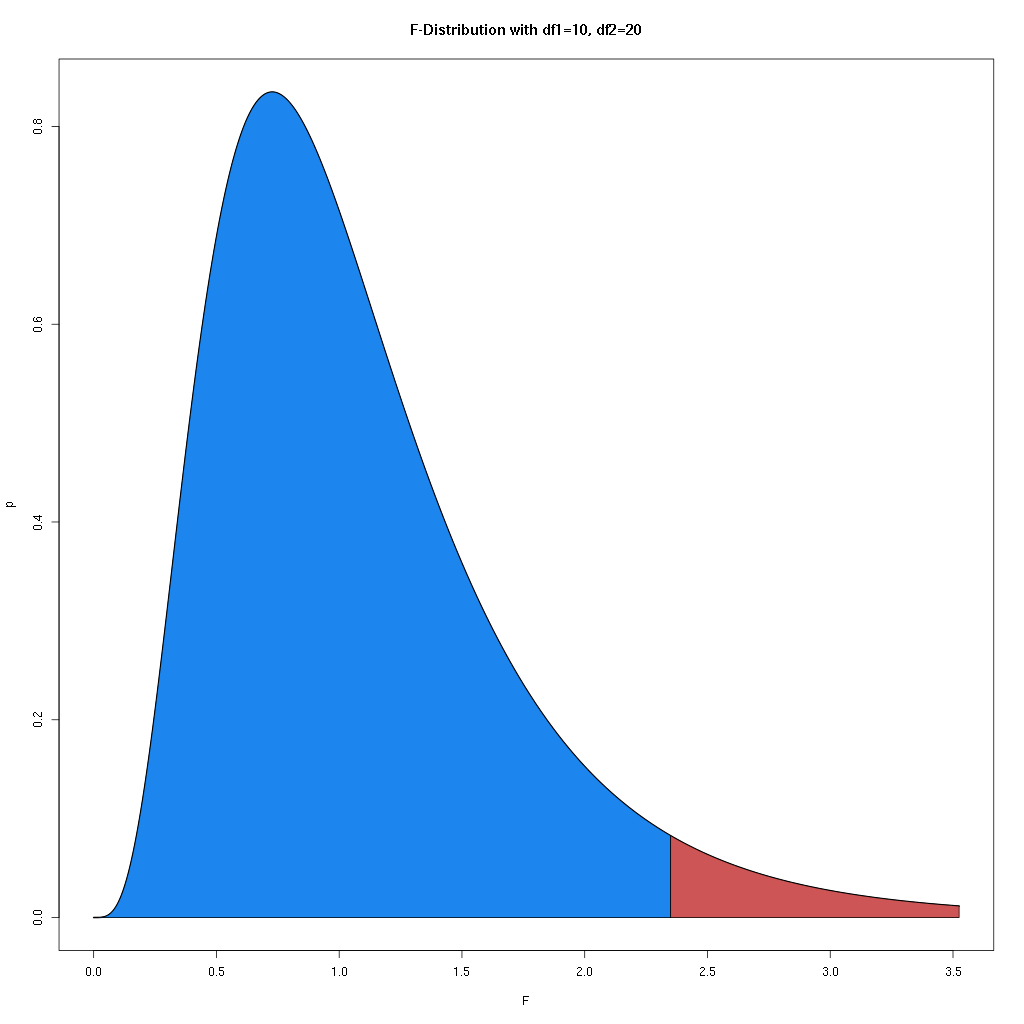
\includegraphics[height=2.0cm]{img/FDistribution}

 {\fontencoding{T1}
 \fontfamily{pcr}
 \fontseries{m}
 \fontshape{n}
 \fontsize{5pt}{5pt}
 \selectfont
\begin{tabular}{l|lllllllllllll} 
df2  & df1      1  &      2  &      3  &      4  &      5  &      6  &      7  &      8  &      9  &     10  &     12  &     15  &     20   \\ 
  1 & 161.4476 & 199.5000 & 215.7073 & 224.5832 & 230.1619 & 233.9860 & 236.7684 & 238.8827 & 240.5433 & 241.8817 & 243.9060 & 245.9499 & 248.0131 \\[5pt] \arrayrulecolor{light-gray}\hline\arrayrulecolor{black}  
  2 & 18.5128 & 19.0000 & 19.1643 & 19.2468 & 19.2964 & 19.3295 & 19.3532 & 19.3710 & 19.3848 & 19.3959 & 19.4125 & 19.4291 & 19.4458 \\[5pt] \arrayrulecolor{light-gray}\hline\arrayrulecolor{black}  
  3 & 10.1280 & 9.5521 & 9.2766 & 9.1172 & 9.0135 & 8.9406 & 8.8867 & 8.8452 & 8.8123 & 8.7855 & 8.7446 & 8.7029 & 8.6602 \\[5pt] \arrayrulecolor{light-gray}\hline\arrayrulecolor{black}  
  4 & 7.7086 & 6.9443 & 6.5914 & 6.3882 & 6.2561 & 6.1631 & 6.0942 & 6.0410 & 5.9988 & 5.9644 & 5.9117 & 5.8578 & 5.8025 \\[5pt] \arrayrulecolor{light-gray}\hline\arrayrulecolor{black}  
  5 & 6.6079 & 5.7861 & 5.4095 & 5.1922 & 5.0503 & 4.9503 & 4.8759 & 4.8183 & 4.7725 & 4.7351 & 4.6777 & 4.6188 & 4.5581 \\[5pt] \arrayrulecolor{light-gray}\hline\arrayrulecolor{black}  
\\ 
  6 & 5.9874 & 5.1433 & 4.7571 & 4.5337 & 4.3874 & 4.2839 & 4.2067 & 4.1468 & 4.0990 & 4.0600 & 3.9999 & 3.9381 & 3.8742 \\[5pt] \arrayrulecolor{light-gray}\hline\arrayrulecolor{black}  
  7 & 5.5914 & 4.7374 & 4.3468 & 4.1203 & 3.9715 & 3.8660 & 3.7870 & 3.7257 & 3.6767 & 3.6365 & 3.5747 & 3.5107 & 3.4445 \\[5pt] \arrayrulecolor{light-gray}\hline\arrayrulecolor{black}  
  8 & 5.3177 & 4.4590 & 4.0662 & 3.8379 & 3.6875 & 3.5806 & 3.5005 & 3.4381 & 3.3881 & 3.3472 & 3.2839 & 3.2184 & 3.1503 \\[5pt] \arrayrulecolor{light-gray}\hline\arrayrulecolor{black}  
  9 & 5.1174 & 4.2565 & 3.8625 & 3.6331 & 3.4817 & 3.3738 & 3.2927 & 3.2296 & 3.1789 & 3.1373 & 3.0729 & 3.0061 & 2.9365 \\[5pt] \arrayrulecolor{light-gray}\hline\arrayrulecolor{black}  
 10 & 4.9646 & 4.1028 & 3.7083 & 3.4780 & 3.3258 & 3.2172 & 3.1355 & 3.0717 & 3.0204 & 2.9782 & 2.9130 & 2.8450 & 2.7740 \\[5pt] \arrayrulecolor{light-gray}\hline\arrayrulecolor{black}  
\\ 
 11 & 4.8443 & 3.9823 & 3.5874 & 3.3567 & 3.2039 & 3.0946 & 3.0123 & 2.9480 & 2.8962 & 2.8536 & 2.7876 & 2.7186 & 2.6464 \\[5pt] \arrayrulecolor{light-gray}\hline\arrayrulecolor{black}  
 12 & 4.7472 & 3.8853 & 3.4903 & 3.2592 & 3.1059 & 2.9961 & 2.9134 & 2.8486 & 2.7964 & 2.7534 & 2.6866 & 2.6169 & 2.5436 \\[5pt] \arrayrulecolor{light-gray}\hline\arrayrulecolor{black}  
 13 & 4.6672 & 3.8056 & 3.4105 & 3.1791 & 3.0254 & 2.9153 & 2.8321 & 2.7669 & 2.7144 & 2.6710 & 2.6037 & 2.5331 & 2.4589 \\[5pt] \arrayrulecolor{light-gray}\hline\arrayrulecolor{black}  
 14 & 4.6001 & 3.7389 & 3.3439 & 3.1122 & 2.9582 & 2.8477 & 2.7642 & 2.6987 & 2.6458 & 2.6022 & 2.5342 & 2.4630 & 2.3879 \\[5pt] \arrayrulecolor{light-gray}\hline\arrayrulecolor{black}  
 15 & 4.5431 & 3.6823 & 3.2874 & 3.0556 & 2.9013 & 2.7905 & 2.7066 & 2.6408 & 2.5876 & 2.5437 & 2.4753 & 2.4034 & 2.3275 \\[5pt] \arrayrulecolor{light-gray}\hline\arrayrulecolor{black}  
\\ 
 16 & 4.4940 & 3.6337 & 3.2389 & 3.0069 & 2.8524 & 2.7413 & 2.6572 & 2.5911 & 2.5377 & 2.4935 & 2.4247 & 2.3522 & 2.2756 \\[5pt] \arrayrulecolor{light-gray}\hline\arrayrulecolor{black}  
 17 & 4.4513 & 3.5915 & 3.1968 & 2.9647 & 2.8100 & 2.6987 & 2.6143 & 2.5480 & 2.4943 & 2.4499 & 2.3807 & 2.3077 & 2.2304 \\[5pt] \arrayrulecolor{light-gray}\hline\arrayrulecolor{black}  
 18 & 4.4139 & 3.5546 & 3.1599 & 2.9277 & 2.7729 & 2.6613 & 2.5767 & 2.5102 & 2.4563 & 2.4117 & 2.3421 & 2.2686 & 2.1906 \\[5pt] \arrayrulecolor{light-gray}\hline\arrayrulecolor{black}  
 19 & 4.3807 & 3.5219 & 3.1274 & 2.8951 & 2.7401 & 2.6283 & 2.5435 & 2.4768 & 2.4227 & 2.3779 & 2.3080 & 2.2341 & 2.1555 \\[5pt] \arrayrulecolor{light-gray}\hline\arrayrulecolor{black}  
 20 & 4.3512 & 3.4928 & 3.0984 & 2.8661 & 2.7109 & 2.5990 & 2.5140 & 2.4471 & 2.3928 & 2.3479 & 2.2776 & 2.2033 & 2.1242 \\[5pt] \arrayrulecolor{light-gray}\hline\arrayrulecolor{black}  
\\ 
 21 & 4.3248 & 3.4668 & 3.0725 & 2.8401 & 2.6848 & 2.5727 & 2.4876 & 2.4205 & 2.3660 & 2.3210 & 2.2504 & 2.1757 & 2.0960 \\[5pt] \arrayrulecolor{light-gray}\hline\arrayrulecolor{black}  
 22 & 4.3009 & 3.4434 & 3.0491 & 2.8167 & 2.6613 & 2.5491 & 2.4638 & 2.3965 & 2.3419 & 2.2967 & 2.2258 & 2.1508 & 2.0707 \\[5pt] \arrayrulecolor{light-gray}\hline\arrayrulecolor{black}  
 23 & 4.2793 & 3.4221 & 3.0280 & 2.7955 & 2.6400 & 2.5277 & 2.4422 & 2.3748 & 2.3201 & 2.2747 & 2.2036 & 2.1282 & 2.0476 \\[5pt] \arrayrulecolor{light-gray}\hline\arrayrulecolor{black}  
 24 & 4.2597 & 3.4028 & 3.0088 & 2.7763 & 2.6207 & 2.5082 & 2.4226 & 2.3551 & 2.3002 & 2.2547 & 2.1834 & 2.1077 & 2.0267 \\[5pt] \arrayrulecolor{light-gray}\hline\arrayrulecolor{black}  
 25 & 4.2417 & 3.3852 & 2.9912 & 2.7587 & 2.6030 & 2.4904 & 2.4047 & 2.3371 & 2.2821 & 2.2365 & 2.1649 & 2.0889 & 2.0075 \\[5pt] \arrayrulecolor{light-gray}\hline\arrayrulecolor{black}  
\\ 
 26 & 4.2252 & 3.3690 & 2.9752 & 2.7426 & 2.5868 & 2.4741 & 2.3883 & 2.3205 & 2.2655 & 2.2197 & 2.1479 & 2.0716 & 1.9898 \\[5pt] \arrayrulecolor{light-gray}\hline\arrayrulecolor{black}  
 27 & 4.2100 & 3.3541 & 2.9604 & 2.7278 & 2.5719 & 2.4591 & 2.3732 & 2.3053 & 2.2501 & 2.2043 & 2.1323 & 2.0558 & 1.9736 \\[5pt] \arrayrulecolor{light-gray}\hline\arrayrulecolor{black}  
 28 & 4.1960 & 3.3404 & 2.9467 & 2.7141 & 2.5581 & 2.4453 & 2.3593 & 2.2913 & 2.2360 & 2.1900 & 2.1179 & 2.0411 & 1.9586 \\[5pt] \arrayrulecolor{light-gray}\hline\arrayrulecolor{black}  
 29 & 4.1830 & 3.3277 & 2.9340 & 2.7014 & 2.5454 & 2.4324 & 2.3463 & 2.2783 & 2.2229 & 2.1768 & 2.1045 & 2.0275 & 1.9446 \\[5pt] \arrayrulecolor{light-gray}\hline\arrayrulecolor{black}  
 30 & 4.1709 & 3.3158 & 2.9223 & 2.6896 & 2.5336 & 2.4205 & 2.3343 & 2.2662 & 2.2107 & 2.1646 & 2.0921 & 2.0148 & 1.9317 \\[5pt] \arrayrulecolor{light-gray}\hline\arrayrulecolor{black}  
\\ 
 31 & 4.1596 & 3.3048 & 2.9113 & 2.6787 & 2.5225 & 2.4094 & 2.3232 & 2.2549 & 2.1994 & 2.1532 & 2.0805 & 2.0030 & 1.9196 \\[5pt] \arrayrulecolor{light-gray}\hline\arrayrulecolor{black}  
 32 & 4.1491 & 3.2945 & 2.9011 & 2.6684 & 2.5123 & 2.3991 & 2.3127 & 2.2444 & 2.1888 & 2.1425 & 2.0697 & 1.9920 & 1.9083 \\[5pt] \arrayrulecolor{light-gray}\hline\arrayrulecolor{black}  
 33 & 4.1393 & 3.2849 & 2.8916 & 2.6589 & 2.5026 & 2.3894 & 2.3030 & 2.2346 & 2.1789 & 2.1325 & 2.0595 & 1.9817 & 1.8977 \\[5pt] \arrayrulecolor{light-gray}\hline\arrayrulecolor{black}  
 34 & 4.1300 & 3.2759 & 2.8826 & 2.6499 & 2.4936 & 2.3803 & 2.2938 & 2.2253 & 2.1696 & 2.1231 & 2.0500 & 1.9720 & 1.8877 \\[5pt] \arrayrulecolor{light-gray}\hline\arrayrulecolor{black}  
 35 & 4.1213 & 3.2674 & 2.8742 & 2.6415 & 2.4851 & 2.3718 & 2.2852 & 2.2167 & 2.1608 & 2.1143 & 2.0411 & 1.9629 & 1.8784 \\[5pt] \arrayrulecolor{light-gray}\hline\arrayrulecolor{black}  
\\ 
 36 & 4.1132 & 3.2594 & 2.8663 & 2.6335 & 2.4772 & 2.3638 & 2.2771 & 2.2085 & 2.1526 & 2.1061 & 2.0327 & 1.9543 & 1.8696 \\[5pt] \arrayrulecolor{light-gray}\hline\arrayrulecolor{black}  
 37 & 4.1055 & 3.2519 & 2.8588 & 2.6261 & 2.4696 & 2.3562 & 2.2695 & 2.2008 & 2.1449 & 2.0982 & 2.0248 & 1.9462 & 1.8612 \\[5pt] \arrayrulecolor{light-gray}\hline\arrayrulecolor{black}  
 38 & 4.0982 & 3.2448 & 2.8517 & 2.6190 & 2.4625 & 2.3490 & 2.2623 & 2.1936 & 2.1375 & 2.0909 & 2.0173 & 1.9386 & 1.8534 \\[5pt] \arrayrulecolor{light-gray}\hline\arrayrulecolor{black}  
 39 & 4.0913 & 3.2381 & 2.8451 & 2.6123 & 2.4558 & 2.3423 & 2.2555 & 2.1867 & 2.1306 & 2.0839 & 2.0102 & 1.9313 & 1.8459 \\[5pt] \arrayrulecolor{light-gray}\hline\arrayrulecolor{black}  
 40 & 4.0847 & 3.2317 & 2.8387 & 2.6060 & 2.4495 & 2.3359 & 2.2490 & 2.1802 & 2.1240 & 2.0772 & 2.0035 & 1.9245 & 1.8389 \\[5pt] \arrayrulecolor{light-gray}\hline\arrayrulecolor{black}  
\\ 
 50 & 4.0343 & 3.1826 & 2.7900 & 2.5572 & 2.4004 & 2.2864 & 2.1992 & 2.1299 & 2.0734 & 2.0261 & 1.9515 & 1.8714 & 1.7841 \\[5pt] \arrayrulecolor{light-gray}\hline\arrayrulecolor{black}  
 60 & 4.0012 & 3.1504 & 2.7581 & 2.5252 & 2.3683 & 2.2541 & 2.1665 & 2.0970 & 2.0401 & 1.9926 & 1.9174 & 1.8364 & 1.7480 \\[5pt] \arrayrulecolor{light-gray}\hline\arrayrulecolor{black}  
 70 & 3.9778 & 3.1277 & 2.7355 & 2.5027 & 2.3456 & 2.2312 & 2.1435 & 2.0737 & 2.0166 & 1.9689 & 1.8932 & 1.8117 & 1.7223 \\[5pt] \arrayrulecolor{light-gray}\hline\arrayrulecolor{black}  
 80 & 3.9604 & 3.1108 & 2.7188 & 2.4859 & 2.3287 & 2.2142 & 2.1263 & 2.0564 & 1.9991 & 1.9512 & 1.8753 & 1.7932 & 1.7032 \\[5pt] \arrayrulecolor{light-gray}\hline\arrayrulecolor{black}  
 90 & 3.9469 & 3.0977 & 2.7058 & 2.4729 & 2.3157 & 2.2011 & 2.1131 & 2.0430 & 1.9856 & 1.9376 & 1.8613 & 1.7789 & 1.6883 \\[5pt] \arrayrulecolor{light-gray}\hline\arrayrulecolor{black}  
\\ 
100 & 3.9361 & 3.0873 & 2.6955 & 2.4626 & 2.3053 & 2.1906 & 2.1025 & 2.0323 & 1.9748 & 1.9267 & 1.8503 & 1.7675 & 1.6764 \\[5pt] \arrayrulecolor{light-gray}\hline\arrayrulecolor{black}  
200 & 3.8884 & 3.0411 & 2.6498 & 2.4168 & 2.2592 & 2.1441 & 2.0556 & 1.9849 & 1.9269 & 1.8783 & 1.8008 & 1.7166 & 1.6233 \\[5pt] \arrayrulecolor{light-gray}\hline\arrayrulecolor{black}  
300 & 3.8726 & 3.0258 & 2.6347 & 2.4017 & 2.2441 & 2.1289 & 2.0402 & 1.9693 & 1.9112 & 1.8623 & 1.7845 & 1.6998 & 1.6057 \\[5pt] \arrayrulecolor{light-gray}\hline\arrayrulecolor{black}  
400 & 3.8648 & 3.0183 & 2.6272 & 2.3942 & 2.2366 & 2.1212 & 2.0325 & 1.9616 & 1.9033 & 1.8544 & 1.7764 & 1.6914 & 1.5969 \\[5pt] \arrayrulecolor{light-gray}\hline\arrayrulecolor{black}  
1000 & 3.8508 & 3.0047 & 2.6138 & 2.3808 & 2.2231 & 2.1076 & 2.0187 & 1.9476 & 1.8892 & 1.8402 & 1.7618 & 1.6764 & 1.5811 \\[5pt] \arrayrulecolor{light-gray}\hline\arrayrulecolor{black}  
\end{tabular}}
\clearpage

Approximation of the critical values for the $F$-distribution for $\alpha=$ 0.02 . 
%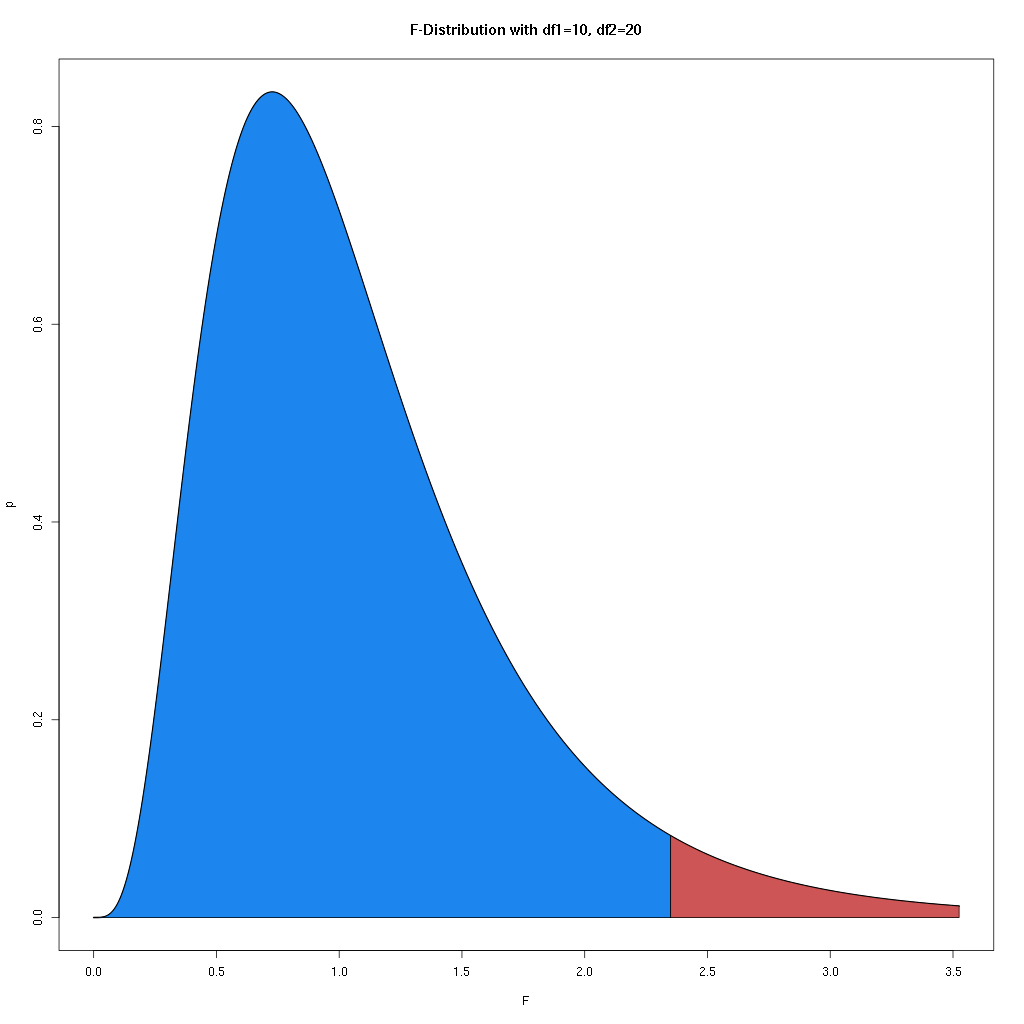
\includegraphics[height=2.0cm]{img/FDistribution}

 {\fontencoding{T1}
 \fontfamily{pcr}
 \fontseries{m}
 \fontshape{n}
 \fontsize{5pt}{5pt}
 \selectfont
\begin{tabular}{l|lllllllllllll} 
df2  & df1      1  &      2  &      3  &      4  &      5  &      6  &      7  &      8  &      9  &     10  &     12  &     15  &     20   \\ 
  1 & 1012.5452 & 1249.5000 & 1350.5047 & 1405.8333 & 1440.6124 & 1464.4548 & 1481.8032 & 1494.9863 & 1505.3405 & 1513.6867 & 1526.3093 & 1539.0545 & 1551.9200 \\[5pt] \arrayrulecolor{light-gray}\hline\arrayrulecolor{black}  
  2 & 48.5051 & 49.0000 & 49.1657 & 49.2487 & 49.2986 & 49.3318 & 49.3556 & 49.3734 & 49.3873 & 49.3984 & 49.4150 & 49.4317 & 49.4483 \\[5pt] \arrayrulecolor{light-gray}\hline\arrayrulecolor{black}  
  3 & 20.6180 & 18.8581 & 18.1097 & 17.6938 & 17.4288 & 17.2451 & 17.1103 & 17.0071 & 16.9256 & 16.8596 & 16.7592 & 16.6571 & 16.5533 \\[5pt] \arrayrulecolor{light-gray}\hline\arrayrulecolor{black}  
  4 & 14.0396 & 12.1421 & 11.3435 & 10.8994 & 10.6157 & 10.4186 & 10.2735 & 10.1622 & 10.0742 & 10.0027 & 9.8939 & 9.7828 & 9.6696 \\[5pt] \arrayrulecolor{light-gray}\hline\arrayrulecolor{black}  
  5 & 11.3228 & 9.4544 & 8.6702 & 8.2330 & 7.9529 & 7.7577 & 7.6137 & 7.5030 & 7.4152 & 7.3438 & 7.2348 & 7.1234 & 7.0094 \\[5pt] \arrayrulecolor{light-gray}\hline\arrayrulecolor{black}  
\\ 
  6 & 9.8764 & 8.0521 & 7.2870 & 6.8594 & 6.5847 & 6.3928 & 6.2508 & 6.1415 & 6.0546 & 5.9839 & 5.8757 & 5.7648 & 5.6509 \\[5pt] \arrayrulecolor{light-gray}\hline\arrayrulecolor{black}  
  7 & 8.9877 & 7.2026 & 6.4539 & 6.0347 & 5.7647 & 5.5756 & 5.4355 & 5.3273 & 5.2413 & 5.1711 & 5.0636 & 4.9531 & 4.8393 \\[5pt] \arrayrulecolor{light-gray}\hline\arrayrulecolor{black}  
  8 & 8.3895 & 6.6366 & 5.9014 & 5.4889 & 5.2227 & 5.0359 & 4.8972 & 4.7900 & 4.7046 & 4.6348 & 4.5278 & 4.4174 & 4.3036 \\[5pt] \arrayrulecolor{light-gray}\hline\arrayrulecolor{black}  
  9 & 7.9605 & 6.2340 & 5.5097 & 5.1027 & 4.8395 & 4.6545 & 4.5169 & 4.4105 & 4.3255 & 4.2561 & 4.1493 & 4.0390 & 3.9249 \\[5pt] \arrayrulecolor{light-gray}\hline\arrayrulecolor{black}  
 10 & 7.6384 & 5.9336 & 5.2182 & 4.8156 & 4.5550 & 4.3714 & 4.2348 & 4.1288 & 4.0442 & 3.9750 & 3.8684 & 3.7581 & 3.6437 \\[5pt] \arrayrulecolor{light-gray}\hline\arrayrulecolor{black}  
\\ 
 11 & 7.3880 & 5.7012 & 4.9932 & 4.5943 & 4.3357 & 4.1533 & 4.0174 & 3.9119 & 3.8275 & 3.7584 & 3.6519 & 3.5415 & 3.4267 \\[5pt] \arrayrulecolor{light-gray}\hline\arrayrulecolor{black}  
 12 & 7.1878 & 5.5163 & 4.8145 & 4.4187 & 4.1617 & 3.9804 & 3.8450 & 3.7398 & 3.6557 & 3.5867 & 3.4802 & 3.3696 & 3.2544 \\[5pt] \arrayrulecolor{light-gray}\hline\arrayrulecolor{black}  
 13 & 7.0241 & 5.3657 & 4.6692 & 4.2760 & 4.0205 & 3.8399 & 3.7050 & 3.6002 & 3.5161 & 3.4472 & 3.3407 & 3.2299 & 3.1143 \\[5pt] \arrayrulecolor{light-gray}\hline\arrayrulecolor{black}  
 14 & 6.8880 & 5.2408 & 4.5488 & 4.1579 & 3.9036 & 3.7237 & 3.5892 & 3.4845 & 3.4006 & 3.3317 & 3.2251 & 3.1142 & 2.9981 \\[5pt] \arrayrulecolor{light-gray}\hline\arrayrulecolor{black}  
 15 & 6.7729 & 5.1354 & 4.4474 & 4.0584 & 3.8052 & 3.6259 & 3.4918 & 3.3873 & 3.3035 & 3.2346 & 3.1279 & 3.0168 & 2.9003 \\[5pt] \arrayrulecolor{light-gray}\hline\arrayrulecolor{black}  
\\ 
 16 & 6.6744 & 5.0455 & 4.3609 & 3.9737 & 3.7214 & 3.5426 & 3.4087 & 3.3044 & 3.2206 & 3.1518 & 3.0450 & 2.9336 & 2.8167 \\[5pt] \arrayrulecolor{light-gray}\hline\arrayrulecolor{black}  
 17 & 6.5892 & 4.9678 & 4.2863 & 3.9006 & 3.6491 & 3.4707 & 3.3371 & 3.2329 & 3.1492 & 3.0803 & 2.9735 & 2.8619 & 2.7446 \\[5pt] \arrayrulecolor{light-gray}\hline\arrayrulecolor{black}  
 18 & 6.5146 & 4.9001 & 4.2213 & 3.8369 & 3.5861 & 3.4081 & 3.2747 & 3.1706 & 3.0869 & 3.0180 & 2.9111 & 2.7993 & 2.6816 \\[5pt] \arrayrulecolor{light-gray}\hline\arrayrulecolor{black}  
 19 & 6.4490 & 4.8404 & 4.1641 & 3.7809 & 3.5307 & 3.3531 & 3.2199 & 3.1159 & 3.0322 & 2.9633 & 2.8563 & 2.7443 & 2.6262 \\[5pt] \arrayrulecolor{light-gray}\hline\arrayrulecolor{black}  
 20 & 6.3907 & 4.7876 & 4.1134 & 3.7313 & 3.4817 & 3.3044 & 3.1713 & 3.0674 & 2.9837 & 2.9148 & 2.8077 & 2.6955 & 2.5770 \\[5pt] \arrayrulecolor{light-gray}\hline\arrayrulecolor{black}  
\\ 
 21 & 6.3386 & 4.7404 & 4.0682 & 3.6870 & 3.4379 & 3.2610 & 3.1280 & 3.0241 & 2.9405 & 2.8716 & 2.7644 & 2.6519 & 2.5331 \\[5pt] \arrayrulecolor{light-gray}\hline\arrayrulecolor{black}  
 22 & 6.2917 & 4.6980 & 4.0276 & 3.6473 & 3.3987 & 3.2220 & 3.0892 & 2.9853 & 2.9017 & 2.8328 & 2.7255 & 2.6128 & 2.4937 \\[5pt] \arrayrulecolor{light-gray}\hline\arrayrulecolor{black}  
 23 & 6.2493 & 4.6597 & 3.9910 & 3.6115 & 3.3633 & 3.1868 & 3.0541 & 2.9503 & 2.8667 & 2.7977 & 2.6904 & 2.5775 & 2.4580 \\[5pt] \arrayrulecolor{light-gray}\hline\arrayrulecolor{black}  
 24 & 6.2109 & 4.6250 & 3.9578 & 3.5790 & 3.3312 & 3.1549 & 3.0223 & 2.9186 & 2.8350 & 2.7660 & 2.6585 & 2.5455 & 2.4257 \\[5pt] \arrayrulecolor{light-gray}\hline\arrayrulecolor{black}  
 25 & 6.1758 & 4.5934 & 3.9275 & 3.5494 & 3.3020 & 3.1259 & 2.9934 & 2.8897 & 2.8060 & 2.7370 & 2.6295 & 2.5163 & 2.3962 \\[5pt] \arrayrulecolor{light-gray}\hline\arrayrulecolor{black}  
\\ 
 26 & 6.1436 & 4.5644 & 3.8998 & 3.5224 & 3.2752 & 3.0993 & 2.9669 & 2.8632 & 2.7796 & 2.7105 & 2.6029 & 2.4895 & 2.3691 \\[5pt] \arrayrulecolor{light-gray}\hline\arrayrulecolor{black}  
 27 & 6.1140 & 4.5378 & 3.8744 & 3.4975 & 3.2507 & 3.0749 & 2.9426 & 2.8389 & 2.7553 & 2.6862 & 2.5785 & 2.4650 & 2.3443 \\[5pt] \arrayrulecolor{light-gray}\hline\arrayrulecolor{black}  
 28 & 6.0868 & 4.5133 & 3.8510 & 3.4746 & 3.2281 & 3.0525 & 2.9202 & 2.8166 & 2.7329 & 2.6638 & 2.5560 & 2.4423 & 2.3214 \\[5pt] \arrayrulecolor{light-gray}\hline\arrayrulecolor{black}  
 29 & 6.0615 & 4.4906 & 3.8293 & 3.4535 & 3.2072 & 3.0317 & 2.8995 & 2.7959 & 2.7122 & 2.6431 & 2.5352 & 2.4214 & 2.3002 \\[5pt] \arrayrulecolor{light-gray}\hline\arrayrulecolor{black}  
 30 & 6.0381 & 4.4696 & 3.8092 & 3.4338 & 3.1878 & 3.0124 & 2.8803 & 2.7767 & 2.6930 & 2.6239 & 2.5159 & 2.4020 & 2.2805 \\[5pt] \arrayrulecolor{light-gray}\hline\arrayrulecolor{black}  
\\ 
 31 & 6.0163 & 4.4500 & 3.7906 & 3.4156 & 3.1698 & 2.9945 & 2.8624 & 2.7589 & 2.6752 & 2.6060 & 2.4980 & 2.3839 & 2.2622 \\[5pt] \arrayrulecolor{light-gray}\hline\arrayrulecolor{black}  
 32 & 5.9960 & 4.4318 & 3.7732 & 3.3986 & 3.1530 & 2.9779 & 2.8458 & 2.7423 & 2.6586 & 2.5894 & 2.4813 & 2.3670 & 2.2451 \\[5pt] \arrayrulecolor{light-gray}\hline\arrayrulecolor{black}  
 33 & 5.9770 & 4.4147 & 3.7569 & 3.3827 & 3.1373 & 2.9623 & 2.8303 & 2.7267 & 2.6430 & 2.5738 & 2.4657 & 2.3513 & 2.2292 \\[5pt] \arrayrulecolor{light-gray}\hline\arrayrulecolor{black}  
 34 & 5.9592 & 4.3987 & 3.7417 & 3.3679 & 3.1226 & 2.9477 & 2.8157 & 2.7122 & 2.6285 & 2.5593 & 2.4510 & 2.3365 & 2.2142 \\[5pt] \arrayrulecolor{light-gray}\hline\arrayrulecolor{black}  
 35 & 5.9425 & 4.3838 & 3.7274 & 3.3539 & 3.1089 & 2.9340 & 2.8021 & 2.6986 & 2.6149 & 2.5456 & 2.4373 & 2.3227 & 2.2001 \\[5pt] \arrayrulecolor{light-gray}\hline\arrayrulecolor{black}  
\\ 
 36 & 5.9268 & 4.3697 & 3.7140 & 3.3408 & 3.0959 & 2.9212 & 2.7893 & 2.6858 & 2.6020 & 2.5328 & 2.4244 & 2.3097 & 2.1869 \\[5pt] \arrayrulecolor{light-gray}\hline\arrayrulecolor{black}  
 37 & 5.9119 & 4.3564 & 3.7013 & 3.3285 & 3.0837 & 2.9090 & 2.7772 & 2.6737 & 2.5900 & 2.5207 & 2.4122 & 2.2974 & 2.1745 \\[5pt] \arrayrulecolor{light-gray}\hline\arrayrulecolor{black}  
 38 & 5.8979 & 4.3439 & 3.6894 & 3.3168 & 3.0722 & 2.8976 & 2.7658 & 2.6623 & 2.5786 & 2.5092 & 2.4008 & 2.2858 & 2.1627 \\[5pt] \arrayrulecolor{light-gray}\hline\arrayrulecolor{black}  
 39 & 5.8847 & 4.3320 & 3.6781 & 3.3058 & 3.0614 & 2.8868 & 2.7550 & 2.6515 & 2.5678 & 2.4984 & 2.3899 & 2.2749 & 2.1516 \\[5pt] \arrayrulecolor{light-gray}\hline\arrayrulecolor{black}  
 40 & 5.8722 & 4.3208 & 3.6674 & 3.2954 & 3.0511 & 2.8766 & 2.7448 & 2.6413 & 2.5576 & 2.4882 & 2.3796 & 2.2645 & 2.1410 \\[5pt] \arrayrulecolor{light-gray}\hline\arrayrulecolor{black}  
\\ 
 50 & 5.7757 & 4.2347 & 3.5854 & 3.2154 & 2.9721 & 2.7981 & 2.6666 & 2.5631 & 2.4793 & 2.4098 & 2.3007 & 2.1847 & 2.0598 \\[5pt] \arrayrulecolor{light-gray}\hline\arrayrulecolor{black}  
 60 & 5.7127 & 4.1785 & 3.5320 & 3.1633 & 2.9207 & 2.7470 & 2.6156 & 2.5122 & 2.4283 & 2.3586 & 2.2492 & 2.1326 & 2.0067 \\[5pt] \arrayrulecolor{light-gray}\hline\arrayrulecolor{black}  
 70 & 5.6682 & 4.1390 & 3.4944 & 3.1267 & 2.8845 & 2.7111 & 2.5798 & 2.4763 & 2.3924 & 2.3226 & 2.2130 & 2.0959 & 1.9691 \\[5pt] \arrayrulecolor{light-gray}\hline\arrayrulecolor{black}  
 80 & 5.6353 & 4.1097 & 3.4666 & 3.0995 & 2.8578 & 2.6845 & 2.5533 & 2.4498 & 2.3658 & 2.2960 & 2.1861 & 2.0687 & 1.9412 \\[5pt] \arrayrulecolor{light-gray}\hline\arrayrulecolor{black}  
 90 & 5.6098 & 4.0871 & 3.4451 & 3.0786 & 2.8371 & 2.6640 & 2.5328 & 2.4293 & 2.3453 & 2.2754 & 2.1654 & 2.0476 & 1.9197 \\[5pt] \arrayrulecolor{light-gray}\hline\arrayrulecolor{black}  
\\ 
100 & 5.5895 & 4.0691 & 3.4281 & 3.0620 & 2.8207 & 2.6477 & 2.5165 & 2.4130 & 2.3290 & 2.2590 & 2.1489 & 2.0309 & 1.9025 \\[5pt] \arrayrulecolor{light-gray}\hline\arrayrulecolor{black}  
200 & 5.4997 & 3.9896 & 3.3526 & 2.9885 & 2.7482 & 2.5756 & 2.4446 & 2.3411 & 2.2568 & 2.1866 & 2.0758 & 1.9566 & 1.8261 \\[5pt] \arrayrulecolor{light-gray}\hline\arrayrulecolor{black}  
300 & 5.4702 & 3.9635 & 3.3279 & 2.9644 & 2.7244 & 2.5520 & 2.4211 & 2.3175 & 2.2332 & 2.1629 & 2.0518 & 1.9322 & 1.8009 \\[5pt] \arrayrulecolor{light-gray}\hline\arrayrulecolor{black}  
400 & 5.4555 & 3.9505 & 3.3156 & 2.9525 & 2.7127 & 2.5403 & 2.4094 & 2.3058 & 2.2214 & 2.1511 & 2.0399 & 1.9201 & 1.7884 \\[5pt] \arrayrulecolor{light-gray}\hline\arrayrulecolor{black}  
1000 & 5.4293 & 3.9274 & 3.2937 & 2.9311 & 2.6916 & 2.5194 & 2.3885 & 2.2849 & 2.2005 & 2.1300 & 2.0186 & 1.8984 & 1.7659 \\[5pt] \arrayrulecolor{light-gray}\hline\arrayrulecolor{black}  
\end{tabular}}
\clearpage

Approximation of the critical values for the $F$-distribution for $\alpha=$ 0.01 . 
% 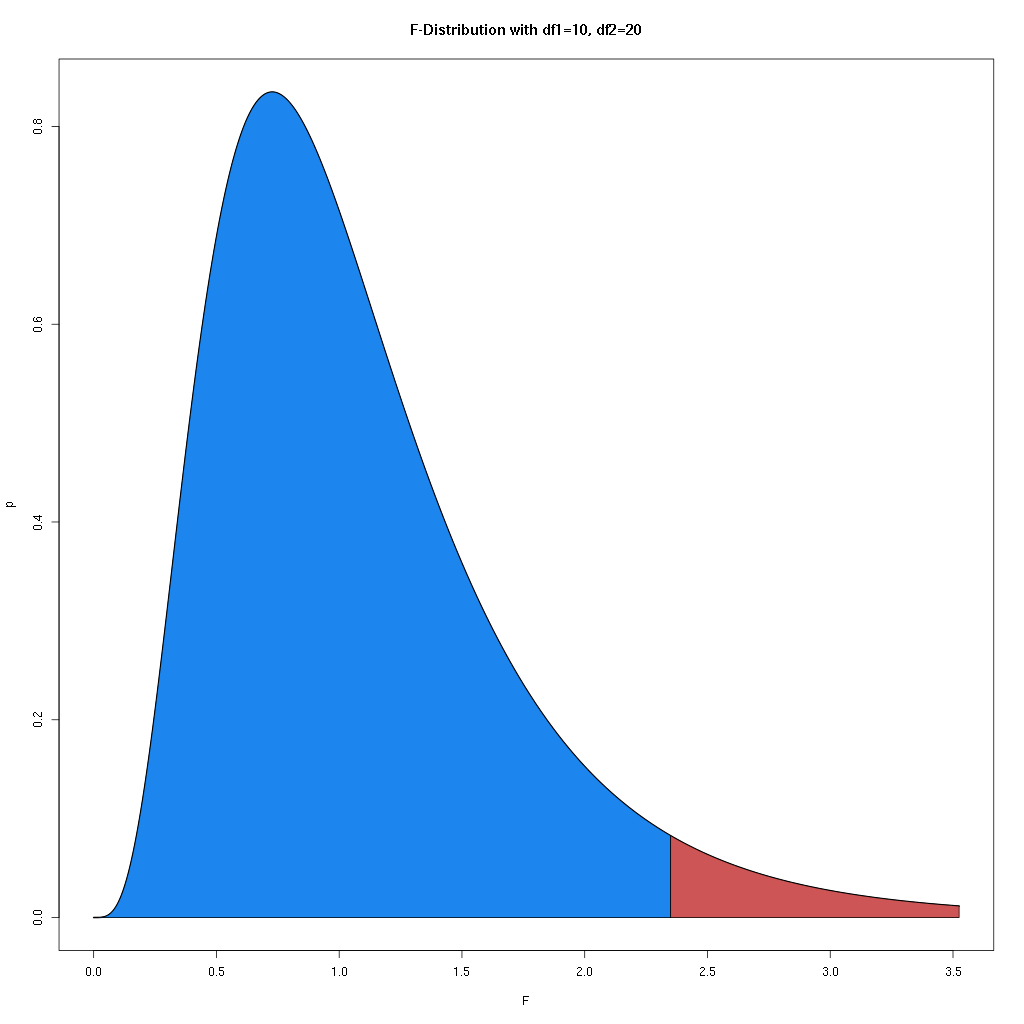
\includegraphics[height=3.0cm]{img/FDistribution}

 {\fontencoding{T1}
 \fontfamily{pcr}
 \fontseries{m}
 \fontshape{n}
 \fontsize{5pt}{5pt}
 \selectfont
\begin{tabular}{l|lllllllllllll} 
df2  & df1      1  &      2  &      3  &      4  &      5  &      6  &      7  &      8  &      9  &     10  &     12  &     15  &     20   \\ 
  1 & 4052.1807 & 4999.5000 & 5403.3520 & 5624.5833 & 5763.6496 & 5858.9861 & 5928.3557 & 5981.0703 & 6022.4732 & 6055.8467 & 6106.3207 & 6157.2846 & 6208.7302 \\[5pt] \arrayrulecolor{light-gray}\hline\arrayrulecolor{black}  
  2 & 98.5025 & 99.0000 & 99.1662 & 99.2494 & 99.2993 & 99.3326 & 99.3564 & 99.3742 & 99.3881 & 99.3992 & 99.4159 & 99.4325 & 99.4492 \\[5pt] \arrayrulecolor{light-gray}\hline\arrayrulecolor{black}  
  3 & 34.1162 & 30.8165 & 29.4567 & 28.7099 & 28.2371 & 27.9107 & 27.6717 & 27.4892 & 27.3452 & 27.2287 & 27.0518 & 26.8722 & 26.6898 \\[5pt] \arrayrulecolor{light-gray}\hline\arrayrulecolor{black}  
  4 & 21.1977 & 18.0000 & 16.6944 & 15.9770 & 15.5219 & 15.2069 & 14.9758 & 14.7989 & 14.6591 & 14.5459 & 14.3736 & 14.1982 & 14.0196 \\[5pt] \arrayrulecolor{light-gray}\hline\arrayrulecolor{black}  
  5 & 16.2582 & 13.2739 & 12.0600 & 11.3919 & 10.9670 & 10.6723 & 10.4555 & 10.2893 & 10.1578 & 10.0510 & 9.8883 & 9.7222 & 9.5526 \\[5pt] \arrayrulecolor{light-gray}\hline\arrayrulecolor{black}  
\\ 
  6 & 13.7450 & 10.9248 & 9.7795 & 9.1483 & 8.7459 & 8.4661 & 8.2600 & 8.1017 & 7.9761 & 7.8741 & 7.7183 & 7.5590 & 7.3958 \\[5pt] \arrayrulecolor{light-gray}\hline\arrayrulecolor{black}  
  7 & 12.2464 & 9.5466 & 8.4513 & 7.8466 & 7.4604 & 7.1914 & 6.9928 & 6.8400 & 6.7188 & 6.6201 & 6.4691 & 6.3143 & 6.1554 \\[5pt] \arrayrulecolor{light-gray}\hline\arrayrulecolor{black}  
  8 & 11.2586 & 8.6491 & 7.5910 & 7.0061 & 6.6318 & 6.3707 & 6.1776 & 6.0289 & 5.9106 & 5.8143 & 5.6667 & 5.5151 & 5.3591 \\[5pt] \arrayrulecolor{light-gray}\hline\arrayrulecolor{black}  
  9 & 10.5614 & 8.0215 & 6.9919 & 6.4221 & 6.0569 & 5.8018 & 5.6129 & 5.4671 & 5.3511 & 5.2565 & 5.1114 & 4.9621 & 4.8080 \\[5pt] \arrayrulecolor{light-gray}\hline\arrayrulecolor{black}  
 10 & 10.0443 & 7.5594 & 6.5523 & 5.9943 & 5.6363 & 5.3858 & 5.2001 & 5.0567 & 4.9424 & 4.8491 & 4.7059 & 4.5581 & 4.4054 \\[5pt] \arrayrulecolor{light-gray}\hline\arrayrulecolor{black}  
\\ 
 11 & 9.6460 & 7.2057 & 6.2167 & 5.6683 & 5.3160 & 5.0692 & 4.8861 & 4.7445 & 4.6315 & 4.5393 & 4.3974 & 4.2509 & 4.0990 \\[5pt] \arrayrulecolor{light-gray}\hline\arrayrulecolor{black}  
 12 & 9.3302 & 6.9266 & 5.9525 & 5.4120 & 5.0643 & 4.8206 & 4.6395 & 4.4994 & 4.3875 & 4.2961 & 4.1553 & 4.0096 & 3.8584 \\[5pt] \arrayrulecolor{light-gray}\hline\arrayrulecolor{black}  
 13 & 9.0738 & 6.7010 & 5.7394 & 5.2053 & 4.8616 & 4.6204 & 4.4410 & 4.3021 & 4.1911 & 4.1003 & 3.9603 & 3.8154 & 3.6646 \\[5pt] \arrayrulecolor{light-gray}\hline\arrayrulecolor{black}  
 14 & 8.8616 & 6.5149 & 5.5639 & 5.0354 & 4.6950 & 4.4558 & 4.2779 & 4.1399 & 4.0297 & 3.9394 & 3.8001 & 3.6557 & 3.5052 \\[5pt] \arrayrulecolor{light-gray}\hline\arrayrulecolor{black}  
 15 & 8.6831 & 6.3589 & 5.4170 & 4.8932 & 4.5556 & 4.3183 & 4.1415 & 4.0045 & 3.8948 & 3.8049 & 3.6662 & 3.5222 & 3.3719 \\[5pt] \arrayrulecolor{light-gray}\hline\arrayrulecolor{black}  
\\ 
 16 & 8.5310 & 6.2262 & 5.2922 & 4.7726 & 4.4374 & 4.2016 & 4.0259 & 3.8896 & 3.7804 & 3.6909 & 3.5527 & 3.4089 & 3.2587 \\[5pt] \arrayrulecolor{light-gray}\hline\arrayrulecolor{black}  
 17 & 8.3997 & 6.1121 & 5.1850 & 4.6690 & 4.3359 & 4.1015 & 3.9267 & 3.7910 & 3.6822 & 3.5931 & 3.4552 & 3.3117 & 3.1615 \\[5pt] \arrayrulecolor{light-gray}\hline\arrayrulecolor{black}  
 18 & 8.2854 & 6.0129 & 5.0919 & 4.5790 & 4.2479 & 4.0146 & 3.8406 & 3.7054 & 3.5971 & 3.5082 & 3.3706 & 3.2273 & 3.0771 \\[5pt] \arrayrulecolor{light-gray}\hline\arrayrulecolor{black}  
 19 & 8.1849 & 5.9259 & 5.0103 & 4.5003 & 4.1708 & 3.9386 & 3.7653 & 3.6305 & 3.5225 & 3.4338 & 3.2965 & 3.1533 & 3.0031 \\[5pt] \arrayrulecolor{light-gray}\hline\arrayrulecolor{black}  
 20 & 8.0960 & 5.8489 & 4.9382 & 4.4307 & 4.1027 & 3.8714 & 3.6987 & 3.5644 & 3.4567 & 3.3682 & 3.2311 & 3.0880 & 2.9377 \\[5pt] \arrayrulecolor{light-gray}\hline\arrayrulecolor{black}  
\\ 
 21 & 8.0166 & 5.7804 & 4.8740 & 4.3688 & 4.0421 & 3.8117 & 3.6396 & 3.5056 & 3.3981 & 3.3098 & 3.1730 & 3.0300 & 2.8796 \\[5pt] \arrayrulecolor{light-gray}\hline\arrayrulecolor{black}  
 22 & 7.9454 & 5.7190 & 4.8166 & 4.3134 & 3.9880 & 3.7583 & 3.5867 & 3.4530 & 3.3458 & 3.2576 & 3.1209 & 2.9779 & 2.8274 \\[5pt] \arrayrulecolor{light-gray}\hline\arrayrulecolor{black}  
 23 & 7.8811 & 5.6637 & 4.7649 & 4.2636 & 3.9392 & 3.7102 & 3.5390 & 3.4057 & 3.2986 & 3.2106 & 3.0740 & 2.9311 & 2.7805 \\[5pt] \arrayrulecolor{light-gray}\hline\arrayrulecolor{black}  
 24 & 7.8229 & 5.6136 & 4.7181 & 4.2184 & 3.8951 & 3.6667 & 3.4959 & 3.3629 & 3.2560 & 3.1681 & 3.0316 & 2.8887 & 2.7380 \\[5pt] \arrayrulecolor{light-gray}\hline\arrayrulecolor{black}  
 25 & 7.7698 & 5.5680 & 4.6755 & 4.1774 & 3.8550 & 3.6272 & 3.4568 & 3.3239 & 3.2172 & 3.1294 & 2.9931 & 2.8502 & 2.6993 \\[5pt] \arrayrulecolor{light-gray}\hline\arrayrulecolor{black}  
\\ 
 26 & 7.7213 & 5.5263 & 4.6366 & 4.1400 & 3.8183 & 3.5911 & 3.4210 & 3.2884 & 3.1818 & 3.0941 & 2.9578 & 2.8150 & 2.6640 \\[5pt] \arrayrulecolor{light-gray}\hline\arrayrulecolor{black}  
 27 & 7.6767 & 5.4881 & 4.6009 & 4.1056 & 3.7848 & 3.5580 & 3.3882 & 3.2558 & 3.1494 & 3.0618 & 2.9256 & 2.7827 & 2.6316 \\[5pt] \arrayrulecolor{light-gray}\hline\arrayrulecolor{black}  
 28 & 7.6356 & 5.4529 & 4.5681 & 4.0740 & 3.7539 & 3.5276 & 3.3581 & 3.2259 & 3.1195 & 3.0320 & 2.8959 & 2.7530 & 2.6017 \\[5pt] \arrayrulecolor{light-gray}\hline\arrayrulecolor{black}  
 29 & 7.5977 & 5.4204 & 4.5378 & 4.0449 & 3.7254 & 3.4995 & 3.3303 & 3.1982 & 3.0920 & 3.0045 & 2.8685 & 2.7256 & 2.5742 \\[5pt] \arrayrulecolor{light-gray}\hline\arrayrulecolor{black}  
 30 & 7.5625 & 5.3903 & 4.5097 & 4.0179 & 3.6990 & 3.4735 & 3.3045 & 3.1726 & 3.0665 & 2.9791 & 2.8431 & 2.7002 & 2.5487 \\[5pt] \arrayrulecolor{light-gray}\hline\arrayrulecolor{black}  
\\ 
 31 & 7.5298 & 5.3624 & 4.4837 & 3.9928 & 3.6745 & 3.4493 & 3.2806 & 3.1489 & 3.0428 & 2.9555 & 2.8195 & 2.6766 & 2.5249 \\[5pt] \arrayrulecolor{light-gray}\hline\arrayrulecolor{black}  
 32 & 7.4993 & 5.3363 & 4.4594 & 3.9695 & 3.6517 & 3.4269 & 3.2583 & 3.1267 & 3.0208 & 2.9335 & 2.7976 & 2.6546 & 2.5029 \\[5pt] \arrayrulecolor{light-gray}\hline\arrayrulecolor{black}  
 33 & 7.4708 & 5.3120 & 4.4368 & 3.9477 & 3.6305 & 3.4059 & 3.2376 & 3.1061 & 3.0003 & 2.9130 & 2.7771 & 2.6341 & 2.4822 \\[5pt] \arrayrulecolor{light-gray}\hline\arrayrulecolor{black}  
 34 & 7.4441 & 5.2893 & 4.4156 & 3.9273 & 3.6106 & 3.3863 & 3.2182 & 3.0868 & 2.9810 & 2.8938 & 2.7580 & 2.6150 & 2.4629 \\[5pt] \arrayrulecolor{light-gray}\hline\arrayrulecolor{black}  
 35 & 7.4191 & 5.2679 & 4.3957 & 3.9082 & 3.5919 & 3.3679 & 3.2000 & 3.0687 & 2.9630 & 2.8758 & 2.7400 & 2.5970 & 2.4448 \\[5pt] \arrayrulecolor{light-gray}\hline\arrayrulecolor{black}  
\\ 
 36 & 7.3956 & 5.2479 & 4.3771 & 3.8903 & 3.5744 & 3.3507 & 3.1829 & 3.0517 & 2.9461 & 2.8589 & 2.7232 & 2.5801 & 2.4278 \\[5pt] \arrayrulecolor{light-gray}\hline\arrayrulecolor{black}  
 37 & 7.3734 & 5.2290 & 4.3595 & 3.8734 & 3.5579 & 3.3344 & 3.1668 & 3.0357 & 2.9302 & 2.8431 & 2.7073 & 2.5642 & 2.4118 \\[5pt] \arrayrulecolor{light-gray}\hline\arrayrulecolor{black}  
 38 & 7.3525 & 5.2112 & 4.3430 & 3.8575 & 3.5424 & 3.3191 & 3.1516 & 3.0207 & 2.9151 & 2.8281 & 2.6923 & 2.5492 & 2.3967 \\[5pt] \arrayrulecolor{light-gray}\hline\arrayrulecolor{black}  
 39 & 7.3328 & 5.1944 & 4.3274 & 3.8425 & 3.5277 & 3.3047 & 3.1373 & 3.0064 & 2.9010 & 2.8139 & 2.6782 & 2.5350 & 2.3824 \\[5pt] \arrayrulecolor{light-gray}\hline\arrayrulecolor{black}  
 40 & 7.3141 & 5.1785 & 4.3126 & 3.8283 & 3.5138 & 3.2910 & 3.1238 & 2.9930 & 2.8876 & 2.8005 & 2.6648 & 2.5216 & 2.3689 \\[5pt] \arrayrulecolor{light-gray}\hline\arrayrulecolor{black}  
\\ 
 50 & 7.1706 & 5.0566 & 4.1993 & 3.7195 & 3.4077 & 3.1864 & 3.0202 & 2.8900 & 2.7850 & 2.6981 & 2.5625 & 2.4190 & 2.2652 \\[5pt] \arrayrulecolor{light-gray}\hline\arrayrulecolor{black}  
 60 & 7.0771 & 4.9774 & 4.1259 & 3.6490 & 3.3389 & 3.1187 & 2.9530 & 2.8233 & 2.7185 & 2.6318 & 2.4961 & 2.3523 & 2.1978 \\[5pt] \arrayrulecolor{light-gray}\hline\arrayrulecolor{black}  
 70 & 7.0114 & 4.9219 & 4.0744 & 3.5996 & 3.2907 & 3.0712 & 2.9060 & 2.7765 & 2.6719 & 2.5852 & 2.4496 & 2.3055 & 2.1504 \\[5pt] \arrayrulecolor{light-gray}\hline\arrayrulecolor{black}  
 80 & 6.9627 & 4.8807 & 4.0363 & 3.5631 & 3.2550 & 3.0361 & 2.8713 & 2.7420 & 2.6374 & 2.5508 & 2.4151 & 2.2709 & 2.1153 \\[5pt] \arrayrulecolor{light-gray}\hline\arrayrulecolor{black}  
 90 & 6.9251 & 4.8491 & 4.0070 & 3.5350 & 3.2276 & 3.0091 & 2.8445 & 2.7154 & 2.6109 & 2.5243 & 2.3886 & 2.2442 & 2.0882 \\[5pt] \arrayrulecolor{light-gray}\hline\arrayrulecolor{black}  
\\ 
100 & 6.8953 & 4.8239 & 3.9837 & 3.5127 & 3.2059 & 2.9877 & 2.8233 & 2.6943 & 2.5898 & 2.5033 & 2.3676 & 2.2230 & 2.0666 \\[5pt] \arrayrulecolor{light-gray}\hline\arrayrulecolor{black}  
200 & 6.7633 & 4.7129 & 3.8810 & 3.4143 & 3.1100 & 2.8933 & 2.7298 & 2.6012 & 2.4971 & 2.4106 & 2.2747 & 2.1294 & 1.9713 \\[5pt] \arrayrulecolor{light-gray}\hline\arrayrulecolor{black}  
300 & 6.7201 & 4.6766 & 3.8475 & 3.3823 & 3.0787 & 2.8625 & 2.6993 & 2.5709 & 2.4668 & 2.3804 & 2.2444 & 2.0988 & 1.9401 \\[5pt] \arrayrulecolor{light-gray}\hline\arrayrulecolor{black}  
400 & 6.6987 & 4.6586 & 3.8309 & 3.3664 & 3.0632 & 2.8472 & 2.6842 & 2.5559 & 2.4518 & 2.3654 & 2.2294 & 2.0836 & 1.9245 \\[5pt] \arrayrulecolor{light-gray}\hline\arrayrulecolor{black}  
1000 & 6.6603 & 4.6264 & 3.8012 & 3.3380 & 3.0355 & 2.8200 & 2.6572 & 2.5290 & 2.4250 & 2.3386 & 2.2025 & 2.0565 & 1.8967 \\[5pt] \arrayrulecolor{light-gray}\hline\arrayrulecolor{black}  
\end{tabular}}


\end{document}
